\chapter{An Introduction to Linear Algebra}

\section{Why Linear Algebra?}
\begin{quote}
    {\bf Of all the mathematical tools that an applied scientist has,\\ \underline{linear algebra is the
    most important.}}
\end{quote}

When a student first encounters linear algebra it may seem like a stretch to call it the
{\it most} important mathematical tool.  That is, until the student relizes that almost
every mathematical operator (such as differentiation, integration, reflection, rotation) and
mathematical process (such as finding a best fit line, solving a system of equations, or
even revealing the frequencies of a sound wave) are all based on the concepts from linear
algebra.  

In this chapter we will take a brief tour of several of the large ideas from linear
algebra to give the reader a flavor of the richness and depth of the topic.  In this
section we will present the {\it three main problems} from linear algebra to highlight the
importance and impact of the field.  Before launching into these problems, the following
problem will give you an introduction to the organizational structure, called a
{\it matrix}, as well as the basic concept of matrix multiplication.

% \input{previews/10.1.PA1}
\begin{problem}
    Advertisements tend to change people's opinions about political issues. Suppose that
    on a certain political issue there are 3 different popular opinions (A, B, and C).  A
    psychologist wants to study the shifts in people's opinions after viewing
    advertisements and hence gathers the data listed in the table below.
    \begin{center}
        \begin{tabular}{|c|c|c|}
            \hline
            Previous Opinion & New Opinion After Viewing Advertisement & Percent Making
            This Switch \\ \hline \hline
            A &A &50\%\\
            A &B &20\%\\
            A &C &30\%\\\hline
            B &A &10\%\\
            B &B &70\%\\
            B &C &20\%\\\hline
            C &A &5\%\\
            C &B &5\%\\
            C &C &90\%\\\hline
        \end{tabular}
    \end{center}

    \begin{enumerate}
        \item[(a)] Create a visual representation of the psychologist's data\footnote{The type
                of visual representation that most people use here is called a {\it graph}
            in mathematics.}.
        \item[(b)] Create a tabular representation of the psychologist's data.
            \begin{center}
                \begin{tabular}{c|ccc}
                    & From A & From B & From C \\ \hline
                    To A &  &  &  \\
                    To B &  &  &  \\
                    To C &  &  &  \\
                \end{tabular}
            \end{center}
        \item[(c)] If there are currently 1200 people in a population with opinion A, 500
            people with opinion B, and 800 with opinion C, then what would the
            psychologist's data predict about the numbers of people with each opinion
            after viewing the advertisements?

        \item[(d)] The psychologist did the study twice, but in an unfortunate instance with a
            hot latte she lost her record of the numbers of people in each category before
            watching the advertisements.  She knows that the end result was 1000 people
            with opinion A, 800 people with opinion B, and 700 people with opinion C.  How
            many people were originally in each category?
    \end{enumerate}
\end{problem}




\subsection*{Systems of Linear Equations: $Ax = b$}
Most people are familiar with systems of linear equations arising from problems in
algebra, business, calculus, and a plethora of other fields.  What is often overlooked in
lower-level mathematics classes is that there is an immense amount of structure embedded
inside a system of equations just waiting to be exploited.  

% \input{activities/10.1.Act1}
\begin{problem}
    Consider a long metal rod that is being heated at one end and held at a constant
    temperature at the other end.  After some time the temperature profile throughout the
    rod will reach a steady state (independent of time).  One way to estimate the steady
    state temperature of the rod is to partition the rod into several equally spaced
    points (see Figure \ref{fig:10.1.rod}) and then to observe that the temperature at a point is the
    average of the temperature of the point to the right and the point to the left.  

    \ba
        \item Write a system of equations associated with the steady state temperature
            profile shown in Figure \ref{fig:10.1.rod}.
        \item Solve the system of equations from part (a) to find the steady state
            temperatures on the rod. You should either use the substitution method or the
            elimination method (which do you think will be more efficient?  more
            organized?).
        \item Now let's go back to the system of equations in part (a) and build a more
            organized description of the problem.  Rearrange the equations so that all of
            the variables are on the left-hand side and all of the corresponding variables
            are aligned vertically. This organization lends itself nicely to a {\it matrix
            equation}, where all of the coefficients are gathered into one matrix, the
            variables into a column vector, and the right-hand sides of the equations in
            another column vector.  Write the system of equations from part (a) as a
            matrix equation.  Explain how this structure lends itself nicely to the
            elimination method.
            \[ \begin{pmatrix} \text{matrix} \\ \text{of} \\ \text{coefficients}
                \end{pmatrix} \cdot \begin{pmatrix} \text{column} \\ \text{of} \\
                    \text{variables} \end{pmatrix} = \begin{pmatrix} \text{right} \\
                        \text{hand}\\ \text{side}  \end{pmatrix} \]
    \ea

    \begin{figure}[ht!]
        \begin{center}
            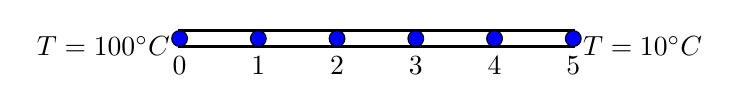
\begin{tikzpicture}
                \draw[very thick, black] (0,0) -- (5,0) -- (5,0.2) -- (0,0.2) -- cycle;
                \foreach \j in {0,1,2,3,4,5}{
                    \draw[fill=blue] (\j,0.1) circle(0.1cm);
                    \draw (\j,0) node[anchor=north]{\j};
                }
                \draw (0,0) node[anchor=east]{$T=100^\circ C$};
                \draw (5,0) node[anchor=west]{$T=10^\circ C$};
            \end{tikzpicture}
        \end{center}
        \caption{A metal rod partitioned into several discrete points.}
        \label{fig:10.1.rod}
    \end{figure}
\end{problem}

\subsection*{Fundamental Matrix Behavior: $Ax = \lambda x$}
The second fundamental problem of linear algebra is to decompose a complicated system of
equations to a collection of elements that are easily visualized.  This is known as the
eigenvector-eigenvalue problem.  In the following activity we will set up a problem that,
without the tools of linear algebra, is very difficult to answer.  We will return to this
example in future sections.

% \input{activities/10.1.Act2}
\begin{problem}
    The female owls in a certain population can be classified as {\it juvenile}, {\it subadult},
    and {\it adult}. In a given year, the number of new juvenile females in year $k+1$ is
    $0.33$ times the  number of adult females in year $k$, 18\% of last year's juveniles become subadults, 71\% of last
    year's subadults become adults, and only 94\% of last year's adults survive.
    \ba
        \item Write a discrete dynamical system for the populations of juveniles $j_k$,
            subadults $s_k$, and adults $a_k$ where $k$ is the year.
        \item Organize the discrete dyamical system into a matrix equation
            \[ \begin{pmatrix} \text{column} \\ \text{of}\\ \text{variables} \\ \text{(time
                = $k+1$)}  \end{pmatrix} = \begin{pmatrix} \text{matrix} \\ \text{of} \\
                \text{coefficients}\\ \text{(time = $k$)} \end{pmatrix} \cdot \begin{pmatrix} \text{column} \\
        \text{of} \\ \text{variables} \\ \text{(time = $k$)} \end{pmatrix}  \]
        \item The owl population will change over time, but it is very important to
            determine ahead of time if the owl popluation is in danger of going extinct.
            Use a spreadsheet program to predict the future of the owl population.  The
            initial populations are not known.
        \item What is the long term behavior of the female owl population?  If you used
            your spreadsheet model from part (c) to make this determination, then how do
            you know that your answer doesn't depend on your chosen intitial conditions?
    \ea

\end{problem}



\subsection*{Least Squares: $A^T A x = A^T b$}
The final of the three big problems from linear algebra is that of least squares curve
fitting.  Instead of {\it least squares}, often times this is referred to as the {\it best
fit line}.  Of course, the word {\it best} is relative to how you measure the error.  In
the following activity you'll set up a best fit line problem with linear algebra.
The techniques to solve the problem will not be covered in this text; this problem is
presented here for completeness of the introduction.

% \input{activities/10.1.Act3}
\begin{problem}
Research on study time vs. exam scores yields the following data points
\begin{center}
    \begin{tabular}{|c|c|}
        \hline
        Time Studying & Exam Score (\%) \\ \hline \hline
        0 & 75 \\
        25 & 70 \\
        30 & 92 \\
        45 & 88 \\
        15 & 90 \\
        30 & 70 \\ \hline
    \end{tabular}
\end{center}

\ba
    \item We would like to find a linear equation of the form $y=ax + b$ where $x$ is the
        time spent studying and $y$ is the exam score.  Write 6 equations where the two
        unknowns are the parameters $a$ and $b$.
    \item Organize your 6 equations into a matrix equation.  The solution to this matrix
        equation is beyond the scope of this chapter, but if we could {\it
        solve}\footnote{Even the word {\it solve} here is arbitrary since there are more
    equations than there are unknowns!} this problem then we would know the slope and
    $y$-intercept that minimize the error between the predictor line and the data.  This
    is a wide reaching topic that will unfortunately have to wait for a different course.
\ea
\end{problem}



\newpage\section{Matrix Operations and Gaussian Elimination} \label{S:10.2.MatrixAlgebra}
One of the first natural questions to ask when first encountering matrices is whether the
regular operations of addition, subtraction, multiplication, division, and exponentiation
make sense.  In the cases of addition and subtraction the answer is simple: Yes!  Addition
and subtraction work in the simplest most natural way with matrices.  The other operations,
on the other hand, need a bit more care but their definitions are robust and immensely
useful.


% \input{previews/10.2.PA1}
\begin{problem}
Consider the matrices 
\[ A = \bpm 1 & 7 & -3 \\ 2 & -3 & 5 \\ 2 & 0 & 1 \epm \quad B = \bpm 3 & -7 & 0 \\ 0 & 0
    & -2 \\ 2 & 4 & 5 \epm \]
\ba
    \item Calculate $A+B$.
    \item Calculate $A-B$.
    \item Calculate $2A$.
\ea
\end{problem}

\subsection*{Matrix Arithmetic}
In this subsection we'll take a brief glimpse at each of the most fundamental matrix
operations as well as some of the foundational definitions for linear algebra.

\begin{definition}[Matrix Arithmetic] Below are several definitions associated with
    matrices.
    \begin{description}
        \item[Size of a Matrix:] If $A$ is a matrix with $m$ rows and $n$ columns then we
            say that $A$ has {\bf size} (or dimensions) $m \times n$.
        \item[Equality:] Two matrices are {\bf equal} if their corresponding entries are
            equal. Matrices can only be equal if the sizes are equal.
        \item[Addition and Subtraction:] Matrix {\bf addition and subtraction} are done by
            regular addition and subtraction on the corresponding entries.  Matrix
            addition and subtraction can only be performed on matrices of the same size.
        \item[Scalar Multiplication:] If $A$ is a matrix then $cA$ is a {\bf scalar
            multiple} of the matrix.  Multiplying a matrix by a scalar multiplies every
            entry by the scalar.
        \item[Transposition:] If $A$ is a matrix then $A^T$ is the {\bf transpose} of the
            matrix found by interchanging the rows and columns of $A$.  If $A$ is $m
            \times n$ then $A^T$ is $n \times m$.
    \end{description}
\end{definition}

The basic operations of addition, subtraction, scalar multiplication, and trasposition all
follow our natural intuition, and we'll get a chance to play with them in the homework.  The
operation of multiplication, on the other hand, takes a bit more care to define.

Before giving a full description of matrix multiplication let us define some very common
notation for matrices.  The size of the matrix is stated by the number of rows then the
number of columns.  This lends itself to a system of double indices for keeping track of
the entries in a matrix. For the matrix $A$ of
size $m \times n$ we denote the individual entry in row $i$ and column $j$ as $a_{ij}$.
In the entire matrix, this becomes
\[ A = \bpm a_{11} & a_{12} & a_{13} & \cdots & a_{1n} \\ 
    a_{21} & a_{22} & a_{23} & \cdots & a_{2n} \\
    \vdots & \vdots & \vdots & \ddots & \vdots \\
    a_{m1} & a_{m2} & a_{m3} & \cdots & a_{mn} \epm \]
So, for example, $a_{37}$ is the entry in row 3 column 7.  More concretely, in the matrix, $A = \bpm 7 & 4 & -2 \\ 3 & 1 & 4 \epm$,
the size is $2 \times 3$ and the entry in row $2$ column $1$ is $a_{21} = 3$.

\begin{definition}
    If $A$ is an $m \times n$ matrix and $B$ is an $n \times p$ matrix then the {\bf
    product} of $A$ and $B$ is $C=AB$.
    \begin{itemize}
        \item The size of $AB$ is $m \times p$.  The number of columns in $A$ must be the
            same as the number of rows of $B$.
        \item The entry in row $i$ and column $j$ of $C=AB$ is
            \[ c_{ij} = a_{i1} b_{1j} + a_{i2} b_{2j} + \cdots + a_{in} b_{nj}. \]
    \end{itemize}

    It is very important to note that in general $AB \ne BA$.
\end{definition}


\begin{example}
Consider the matrices $A$ and $B$ defined as 
\[ A = \bpm 1 & 2 & -3 \\ 2 & 0 & 1 \epm \quad \text{and} \quad  B=\bpm 5 & -2 \\ -1 & 0 \\ 1 & 3 \epm. \]
Find $AB$ and $BA$ if they exist.
\\{\bf Solution:}
First note that $A$ is a $2 \times 3$ matrix and $B$ is a $3 \times 2$ matrix.  Hence,
$AB$ will be $2 \times 2$ and $BA$ will be $3 \times 3$. \footnote{If you read this
    example without picking up your pencil and trying the example then you may want to
pause and rethink your decisions.  Mathematics is not a spectator's sport!}
\begin{flalign*}
    AB &= \bpm 1 & 2 & -3 \\ 2 & 0 & 1 \epm \bpm 5 & -2 \\ -1 & 0 \\ 1 & 3 \epm \\
    %
    &= \bpm 1\cdot 5 + 2 \cdot (-1) +(-3)\cdot 1 & 1 \cdot (-2) + 2 \cdot 0 + (-3) \cdot 3
    \\ 2 \cdot 5 + 0 \cdot (-1) + \cdot 1 \cdot 1 & 2 \cdot (-2) + 0 \cdot 0 + 1 \cdot 3
    \epm \\
    %
    &= \bpm 0 & -11 \\ 11 & -1 \epm
\end{flalign*}
To be very clear about the process, the $-11$ in row 1 column 2 of the answer came from
multiplying the corresponding entries of row 1 of matrix $A$ by column 2 of matrix $B$ and
finding the sum of the products.

\begin{flalign*}
    BA &= \bpm 5 & -2 \\ -1 & 0 \\ 1 & 3 \epm \bpm 1 & 2 & -3 \\ 2 & 0 & 1 \epm \\
    %
    &= \bpm 5\cdot1 + (-2) \cdot 2 & 5 \cdot 2 + (-2) \cdot 0 & 5 \cdot (-3) + (-2) \cdot 1 \\
    (-1)\cdot1 + 0 \cdot 2 & (-1) \cdot 2 + 0 \cdot 0 & (-1) \cdot (-3) + 0 \cdot 1 \\
    1\cdot1 + 3 \cdot 2 & 1 \cdot 2 + 3 \cdot 0 & 1 \cdot (-3) + 3 \cdot 1
    \epm \\
    %
    &= \bpm 1 & 10 & -17 \\ -1 & -2 & 3 \\ 7 & 2 & 0 \epm
\end{flalign*}
\end{example}




% \input{activities/10.2.Act1}
\begin{problem}
Consider the matrices
\[ A = \bpm 2 & -1 & 4 \\ 3 & 0 & 1 \epm, \quad B = \bpm 2 & 1 \\ 0 & -3 \\ 4 & -1 \epm,
    \quad C = \bpm 0 & -1 \\ 3 & 2 \\ -2 & 1 \epm, \quad \text{and} \quad \bx =
    \bpm 1 \\ 3 \\ -2 \epm. \]
\ba
    \item Determine which products are possible: $AB$, $AC$, $A\bx$, $BA$,
        $CA$, $\bx A$, $BC$, $B\bx$, $CB$, $C\bx$. For
        each of the products that is possible, find the size of the result.
    \item Write the product $AB$ and the product $BA$.  Does $AB = BA$?
\ea
\end{problem}

\newpage\section{Gaussian Elimination: A First Look At Solving Systems}
A truly beautiful application of matrices, and the first real application of linear
algebra, is the technique of solving systems of linear equations.  The technique that
we'll describe in the next several activities and examples is used to solve systems of
equations in a very organized fashion.  Most students are familiar with the {\it
elimination method} from high school algebra, and the technique of {\it Gaussian
Elimination} described herein is simply a more organized way to perform the exact same
technique.  You'll find that systems of linear equations arise naturally in all sorts of
applications so we include this as one of the essential tools for mathematical modeling.


\begin{example}
Consider the following system of equations. 
    \begin{flalign}
        \notag -x_1 + x_2 - x_3 &= 1 \\
        3x_2 + 2x_3 &= -8 \label{eqn:S10.2:system1} \\
        \notag x_3 &= 2
    \end{flalign}
Solve the system algebraically and reorganize the system using the powerful and beautiful
structure of matrices \footnote{If you haven't notice, the author loves matrices!}
\\{\bf Solution:}
Any technique for solving systems will suffice.  This particular system is set up to
reveal a solution quickly.  Indeed, it is obvious that $x_3=2$.  Using this fact, the
second equation can be rewritten and solved as
\[ 3x_2 + 2(2) = -8 \quad \implies \quad 3x_2 = -12 \quad \implies \quad x_2 = -4. \]
Now that we have both $x_2$ and $x_3$ the first equation can be rewritten as solved as
\[ -x_1 + (-4) - (2) = 1 \quad \implies \quad -x_1 = 7 \quad \implies \quad x_1 = -7 \]

Now we'll leverage the organizational power of matrices:\\
The system of equations can be written in matrix form as 
\begin{flalign}
    \bpm -1 & 1 & -1 \\ 0 & 3 & 2 \\ 0 & 0 & 1 \epm \bpm x_1 \\ x_2 \\ x_3 \epm = \bpm 1 \\
    -8 \\ 2 \epm 
    \label{eqn:S10.2:system1b}
\end{flalign}
Multiplying the $3 \times 3$ matrix on the left-hand side by the $3 \times 1$ vector
$\bpm x_1 \\ x_2 \\ x_3 \epm$ reveals that the matrix equation in
\eqref{eqn:S10.2:system1b} is indeed the same as the system of equations in
\eqref{eqn:S10.2:system1}. This important observation illustrated that we can take any
system of linear equations and write it in such a way.
        
The matrix equation can be further reorganized into an {\it augmented
system}:
\[ \left( \begin{array}{ccc|c} -1 & 1 & -1 & 1 \\ 0 & 3 & 2 & -8 \\ 0 & 0 & 1 & 2
    \end{array} \right) \]
This is simply an organizational technique and we use it because the names of
the variables are arbitrary and irrelevant to the solution. The first line of the
augmented system can be read as $-x_1 + x_2 - x_3 = 1$ where the variables are inferred
and only inserted when necessary.  The last line of the augmented
system can be read as $0 x_1 + 0 x_2 + x_3 = 2$, so this clearly reveals that $x_3 = 2$.
\end{example}

% \input{activities/10.2.Act2}
\begin{problem}
    In this activity we wish to solve the system of equations.
    \begin{flalign*}
        -x_1 + x_2 - x_3 &= -6 \\
        x_1 + x_3 &= 15 \\
        2x_1 - x_2 + x_3 &= 9
    \end{flalign*}
    We will do so in a very structured and organized fashion to illustrate the {\it
    Gaussian Elimination} technique for solving systems.
    \ba
        \item First write the system as a matrix equation.
            \[ \bpm \underline{\hspace{0.25in}} & \underline{\hspace{0.25in}} &\underline{\hspace{0.25in}} \\
            \underline{\hspace{0.25in}} & \underline{\hspace{0.25in}} &\underline{\hspace{0.25in}} \\
            \underline{\hspace{0.25in}} & \underline{\hspace{0.25in}}
            &\underline{\hspace{0.25in}} \epm \bpm x_1 \\ x_2 \\ x_3 \epm = \bpm
            \underline{\hspace{0.25in}} \\ \underline{\hspace{0.25in}} \\ 
            \underline{\hspace{0.25in}} \epm \]
        \item Now write the system as an {\it augmented system}
            \[ \left( \begin{array}{ccc|c}
                \underline{\hspace{0.25in}} & \underline{\hspace{0.25in}} &\underline{\hspace{0.25in}} &\underline{\hspace{0.25in}} \\
                \underline{\hspace{0.25in}} & \underline{\hspace{0.25in}} &\underline{\hspace{0.25in}} &\underline{\hspace{0.25in}} \\
                \underline{\hspace{0.25in}} & \underline{\hspace{0.25in}} &\underline{\hspace{0.25in}} &\underline{\hspace{0.25in}} \\
            \end{array} \right) \]
        \item Using the operations:
            \begin{itemize}
                \item multiply one row by a scalar quantity
                \item add a multiple of one row to another row
                \item interchange two rows
            \end{itemize}
            we wish to transform the augmented system you wrote in part (b) to something
            of the form
            \[ \left( \begin{array}{ccc|c} 1 & 0 & 0 & \star \\ 0 & 1 & 0 & \star \\ 0 & 0
                & 1 & \star \end{array} \right) \]
            Discuss with your partners why the above operations are mathematically valid.
        \item Work with your partners to discuss the first and most logical operation to do
            that will move you toward that direction.
        \item Use the operations outlined in part (c) to solve the system.  Pay particular
            attention to the order in which you perform the row reduction.
    \ea
\end{problem}

\begin{definition}
    The {\bf Gaussian Elimination} technique (also called {\bf row reduction}) is an
    algorithm used to perform the elimination method on a system of linear equations of
    virtually any size.
    \begin{enumerate}
        \item Write the system of equations in augmented form.
        \item Perform row operations to get to a triangular system of equations.  The row
            operations allowed are:
            \begin{itemize}
                \item Multiply a row by any nonzero number.
                \item Add a multiple of one row to another.
                \item Interchange two rows.
            \end{itemize}
        \item Once the system is written in triangular form, either back substitute to solve the
            system or continue performing row operations to arrive at the form
            \[ \left( \begin{array}{ccccc|c} 1 & 0 & 0 & \cdots & 0 & \star \\
                    0 & 1 & 0 & \cdots & 0 & \star \\
                    0 & 0 & \ddots & \cdots & 0 & \star \\
                    \vdots & \vdots & \cdots & \ddots & \vdots & \vdots \\
                    0 & 0 & 0 & \cdots & 1 & \star \end{array} \right) \]
            At which point, read the answer from the augmented form.
    \end{enumerate}
\end{definition}

Next we will show a fully worked example of Gaussian Elimination in action to give some
hints to the thought process that goes on behind the scenes.  


\begin{example}
Solve the system of equations
\begin{flalign*}
    x_1 + 0 x_2 + 3x_3 + 2x_4 &= -20 \\
    0 x_1 + x_2 - 4x_3 - 4x_4 &= 32 \\
    2x_1 - 3x_2 + 16x_3 + 16x_4 &= -120 \\
    0 x_1 - x_2 + 4x_3 + 9x_4 &= -27
\end{flalign*}
{\bf Solution:}
If we first write this as an augmented matrix we get
\[ \left( \begin{array}{cccc|c} 
        1 & 0 & 3 & 2 & -20 \\
        0 & 1 & -4 & -4 & 32 \\
        2 & -3 & 16 & 16 & -120 \\
        0 & -1 & 4 & 9 & -27 \end{array} \right). \]
Next we start performing row operations with the goal of creating a triangular system. The
observant reader will notice that, while this system of equations can be solved with any
(non-graphical) technique from high school algebra, the Gaussian Elimination technique is
far more organized.

Add $(-2)$ times row 1 to row 3. Put the answer in row 3.
\[ % \left( \begin{array}{cccc|c} 
%         1 & 0 & 3 & 2 & -20 \\
%         0 & 1 & -4 & -4 & 32 \\
%         2 & -3 & 16 & 16 & -120 \\
%         0 & -1 & 4 & 9 & -27 \end{array} \right) 
        \stackrel{-2R_1 + R_3}{\longrightarrow}
    \left( \begin{array}{cccc|c} 
        1 & 0 & 3 & 2 & -20 \\
        0 & 1 & -4 & -4 & 32 \\
        0 & -3 & 10 & 12 & -80 \\
        0 & -1 & 4 & 9 & -27 \end{array} \right)    
        \]

Add $(3)$ times row 2 to row 3. Put the answer in row 3.
\[ % \left( \begin{array}{cccc|c} 
%         1 & 0 & 3 & 2 & -20 \\
%         0 & 1 & -4 & -4 & 32 \\
%         0 & -3 & 10 & 12 & -80 \\
%         0 & -1 & 4 & 9 & -27 \end{array} \right) 
        \stackrel{3R_2 + R_3}{\longrightarrow}
    \left( \begin{array}{cccc|c} 
        1 & 0 & 3 & 2 & -20 \\
        0 & 1 & -4 & -4 & 32 \\
        0 & 0 & -2 & 0 & 16 \\
        0 & -1 & 4 & 9 & -27 \end{array} \right)    
        \]

Add $(1)$ times row 2 to row 4. Put the answer in row 4.
\[%  \left( \begin{array}{cccc|c} 
%         1 & 0 & 3 & 2 & -20 \\
%         0 & 1 & -4 & -4 & 32 \\
%         0 & 0 & -2 & 0 & 16 \\
%         0 & -1 & 4 & 9 & -27 \end{array} \right) 
        \stackrel{(1)R_2 + R_4}{\longrightarrow}
    \left( \begin{array}{cccc|c} 
        1 & 0 & 3 & 2 & -20 \\
        0 & 1 & -4 & -4 & 32 \\
        0 & 0 & -2 & 0 & 16 \\
        0 & 0 & 0 & 5 & 5 \end{array} \right)    
        \]

Divide row 3 by $(-2)$ and put the answer in row 3.
\[%  \left( \begin{array}{cccc|c} 
%         1 & 0 & 3 & 2 & -20 \\
%         0 & 1 & -4 & -4 & 32 \\
%         0 & 0 & -2 & 0 & 16 \\
%         0 & 0 & 0 & 5 & 5 \end{array} \right) 
        \stackrel{R_3/(-2)}{\longrightarrow}
    \left( \begin{array}{cccc|c} 
        1 & 0 & 3 & 2 & -20 \\
        0 & 1 & -4 & -4 & 32 \\
        0 & 0 & 1 & 0 & -8 \\
        0 & 0 & 0 & 5 & 5 \end{array} \right)    
        \]

Divide row 4 by 5 to arrive at a triangular form.
\[% \left( \begin{array}{cccc|c} 
%         1 & 0 & 3 & 2 & -20 \\
%         0 & 1 & -4 & -4 & 32 \\
%         0 & 0 & 1 & 0 & -8 \\
%         0 & 0 & 0 & 5 & 5 \end{array} \right) 
        \stackrel{R_4/5}{\longrightarrow}
    \left( \begin{array}{cccc|c} 
        1 & 0 & 3 & 2 & -20 \\
        0 & 1 & -4 & -4 & 32 \\
        0 & 0 & 1 & 0 & -8 \\
        0 & 0 & 0 & 1 & 1 \end{array} \right)    
        \]

Now that this is in triangular form you can back substitute or simply continue performing
row operations.  We will choose to perform the row operations to determine the solution.

 
\[ \stackrel{4R_3+R_2, \, 4R_4+R_2}{\longrightarrow} \left( \begin{array}{cccc|c}
        1 & 0 & 3 & 2 & -20 \\
        0 & 1 & 0 & 0 & 4 \\
        0 & 0 & 1 & 0 & -8 \\
        0 & 0 & 0 & 1 & 1 \end{array} \right)
\stackrel{(-3)R_3+R_1, \, (-2)R_4+R_1}{\longrightarrow} \left( \begin{array}{cccc|c}
        1 & 0 & 0 & 0 & 2 \\
        0 & 1 & 0 & 0 & 4 \\
        0 & 0 & 1 & 0 & -8 \\
        0 & 0 & 0 & 1 & 1 \end{array} \right)
        \]

After all of this simplification, the final solution is 
\[ \boxed{x_1 = 2, \, x_2 = 4, \, x_3 = -8, \, x_4 = 1} \]
\end{example}

The process of performing Gaussian Elimination may take a lot of paper, but once you get
the hang of the process it is far more organized than any other technique for solving
systems of linear equations.  

\begin{technique}[Practical Tips for Gaussian Elimination]
You should use the following tips for doing Gaussian Elimination.
\begin{itemize}
    \item First try to get a 1 in the upper left-hand corner of the augmented matrix.
    \item Next, use the new first row to eliminate all of the non-zero entries in the
        first column.  By the time you're done with this you should have a column with a 1
        on top and zeros below.
    \item Next get a 1 in row 2 column 2.
    \item Use your new second row to eliminate all of the non-zero entries in the second
        column.
    \item Proceed in a similar fashion until you have reached the final row.
\end{itemize}
\end{technique}

% \input{activities/10.2.Act3}
\begin{problem}
Write the following system in augmented form and use Gaussian Elimination to solve for
$x_1$, $x_2$, and $x_3$.
    \begin{flalign*}
        x_1 - 2 x_2 + x_3 &= 0 \\
        2x_2 - 8 x_3 &= 8 \\
        -4x_1 + 5x_2 + 9x_3 &= -9
    \end{flalign*}
\end{problem}



\newpage\section{Systems of Linear Equations} \label{S:10.3.Systems}

In this section we further explore the notion of solving a linear system of equations. To
begin our study consider the following Preview Activity.

% \input{previews/10.3.PA1}
\begin{problem}
    Solve each of the three systems of two equations and two unknowns.  One of the systems
    has infinitely many solutions, one of the systems has exactly one solution, and one of
    the systems has no solutions.  In each case, use augmented matrices and Gaussian
    Elimination to solve the system.
    \ba
        \item Solve the system
            \begin{flalign*}
                x_1 - 2 x_2 &= 4 \\
                -2x_1+4x_2 &= 5
            \end{flalign*}

        \item Solve the system
            \begin{flalign*}
                x_1 - 2 x_2 &= 4 \\
                -2x_1+4x_2 &= -8
            \end{flalign*}

        \item Solve the system
            \begin{flalign*}
                x_1 - 2 x_2 &= 4 \\
                2x_1 + 4x_2 &= 5
            \end{flalign*}
    \ea
\end{problem}

\subsection*{Systems, Matrix Equations, and Vector Equations}
A system of linear equations can always be written in several different ways.  The most
familiar of which is the collection of equations themselves.  The three other ways to
write a system of equations are the {\bf matrix form}, the {\bf vector form}, and the {\bf
augmented matrix form}.  

Consider the system of $m$ linear equations with $n$ unknowns
\begin{flalign}
    \notag a_{11} x_1 + a_{12} x_2 + \cdots + a_{1n} x_n &= b_1 \\
    \notag a_{21} x_1 + a_{22} x_2 + \cdots + a_{2n} x_n &= b_2 \\
    \notag a_{31} x_1 + a_{32} x_2 + \cdots + a_{3n} x_n &= b_3 \\
    \notag & \vdots \\
    a_{m1} x_1 + a_{m2} x_2 + \cdots + a_{mn} x_n &= b_m \label{eqn:10.3.system}
\end{flalign}

\begin{definition}
    The {\bf matrix form} of the system of equations \eqref{eqn:10.3.system} is
    \[ \bpm a_{11} & a_{12} & \cdots & a_{1n} \\
        a_{21} & a_{22} & \cdots & a_{2n} \\
        a_{31} & a_{32} & \cdots & a_{3n} \\
        \vdots & \vdots & \ddots & \vdots \\
        a_{m1} & a_{m2} & \cdots & a_{mn} \epm 
        \bpm x_1 \\ x_2 \\ x_3 \\ \vdots \\ x_n \epm
        =
        \bpm b_1 \\ b_2 \\ b_3 \\ \vdots \\ b_m \epm
        \]
    In symbols, this is denoted $A \bx = \bb$.
\end{definition}

\begin{definition}
    The {\bf vector form} of the system of equations \eqref{eqn:10.3.system} is
    \[ x_1 \bpm a_{11} \\ a_{21} \\ a_{31} \\ \vdots \\ a_{m1} \epm + 
        x_2 \bpm a_{12} \\ a_{22} \\ a_{32} \\ \vdots \\ a_{m2} \epm +
        x_3 \bpm a_{13} \\ a_{23} \\ a_{33} \\ \vdots \\ a_{m3} \epm + \cdots
        x_n \bpm a_{1n} \\ a_{2n} \\ a_{3n} \\ \vdots \\ a_{mn} \epm =
        \bpm b_1 \\ b_2 \\ b_3 \\ \vdots \\ b_m \epm
        \]
        In symbols, this is denoted $x_1 \texttt{a}_1 + x_2 \texttt{a}_2 + x_3 \texttt{a}_3 + \cdots + x_n
        \texttt{a}_n = \texttt{b}$.
\end{definition}

\begin{definition}
    The {\bf augmented form} of the system of equation \eqref{eqn:10.3.system} is
    \[ \left( \begin{array}{ccccc|c}
            a_{11} & a_{12} & a_{13} & \cdots & a_{1n} & b_1 \\
            a_{21} & a_{32} & a_{33} & \cdots & a_{3n} & b_3 \\
            a_{31} & a_{32} & a_{33} & \cdots & a_{3n} & b_3 \\
            \vdots & \vdots & \vdots & \ddots & \vdots & \vdots \\
            a_{m1} & a_{m2} & a_{m3} & \cdots & a_{mn} & b_m 
        \end{array} \right)
            \]
            In symbols this is denoted $(A | \texttt{b})$.
\end{definition}

% Throughout the remainder of this chapter, a bold symbol will denote a vector and a capital
% letter will denote a matrix.  This is common notation in the study of linear algebra and
% it allows us to distinguish between scalar quantities, vector quantities, and matrices.


\subsection*{Solution Sets to Systems of Equations}
It is not guaranteed that a system of equations will have a solution.  Moreover, if there
is a solution it is not guaranteed that the solution will be unique. Theorem
\ref{thm:10.3.exist_unique} gives the conditions for which a system of linear equations
will have no solutions, infinitely many solutions, or exactly one solution.

\begin{thm}
    \begin{enumerate}
        \item A system of linear equations has no solutions if after it is row reduced it
            has a row of the form
            \[ \bpm 0 & 0 & \cdots & 0 & | & \star \epm \]
            where the number $\star$ is nonzero.  This row in the reduced matrix is
            equivalent to saying that $0 = \star$; which is never true.
        \item A system of linear equations has one unique solution if at the end of the
            row reduction one can determine every variable.
        \item A system of linear equations has infinitely many solutions if at the end of
            the row reduction there are variables that you cannot determine uniquely.
    \end{enumerate}
    \label{thm:10.3.exist_unique}
\end{thm}


% 
% \input{activities/10.3.Act1}
\begin{problem}\label{A:10.3.1}
\ba 
\item Consider the following augmented matrices in reduced row echelon form.  Determine the
number of solutions. If there is one unique solution then find it.
\begin{itemize}
    \item[(i)] 
        \[ \left( \begin{array}{ccc|c} 
                1 & 0 & 0 & 3 \\
                0 & 1 & 0 & 2 \\
                0 & 0 & 1 & -5 \end{array} \right) \]
            \item[(ii)] 
        \[ \left( \begin{array}{ccc|c} 
                1 & 0 & 0 & 3 \\
                0 & 1 & 0 & 2 \\
                0 & 0 & 0 & -5 \end{array} \right) \]
            \item[(iii)]
        \[ \left( \begin{array}{ccc|c} 
                1 & 0 & 1 & 3 \\
                0 & 1 & 0 & 2 \\
                0 & 0 & 0 & 0 \end{array} \right) \]
        \end{itemize}

    \item Determine the value of $h$ such that the matrix is the augmented matrix of a
        linear system with infinitely many solutions
        \[ \left( \begin{array}{cc|c} 3 & -4 & 4 \\ 9 & h & 12 \end{array} \right) \]
\ea
\end{problem}


In Activity \ref{A:10.3.1}, problem (a) part (iii) has infinitely many solutions.  In
order to find a complete description of those solutions we can rewrite the problem in
terms of the variables to get 
\begin{flalign*}
    x_1 + x_3 &= 3 \\
    x_2 &= 2.
\end{flalign*}
It is obvious from this description that $x_2$ is fixed at $2$, but the values of $x_1$
and $x_3$ depend on each other.  In cases like this we choose one variable to be a {\it
parameter} and express the
other variable in terms of that parameter.  In this case, we let $x_3 = t$ and we can write the first equation
as
\[ x_1 = 3- t \]
Since $t$ can take on any real value we finally write the solution as 
\[ x_1 = 3-t \quad \text{and} \quad x_2 = 2 \quad \text{where} \quad x_3=t \quad
    \text{and} \quad -\infty < t < \infty. \]

Written as a vector, the solution is
\[ \bpm x_1 \\ x_2 \\ x_3 \epm = \bpm 3 \\ 2 \\ 0 \epm + \bpm -1 \\ 0 \\ 1 \epm t. \]

In two and three dimensions there are nice geometric interpretations for these types of
solutions.
\begin{example}
Consider the following three systems of equations and their row reduced forms.  Describe
their solution sets geometrically.
\begin{flalign*}
    \text{System \#1:} & \left( \begin{array}{cc|c} 1 & -1 & 3 \\ 2 & 1 & 0 \end{array}
        \right) \to \cdots \to \left( \begin{array}{cc|c} 1 & 0 & 1 \\ 0 & 1 & -2
        \end{array} \right) \\
    %
    \text{System \#2:} & \left( \begin{array}{cc|c} 1 & -1 & 3 \\ -1 & 1 & 0 \end{array}
        \right) \to \cdots \to \left( \begin{array}{cc|c} 1 & -1 & 3 \\ 0 & 0 & 3
        \end{array} \right) \\
  %
    \text{System \#3:} & \left( \begin{array}{cc|c} 1 & -1 & 3 \\ -1 & 1 & -3 \end{array}
        \right) \to \cdots \to \left( \begin{array}{cc|c} 1 & -1 & 3 \\ 0 & 0 & 0
        \end{array} \right) 
\end{flalign*}
{\bf Solution:}
Figure \ref{fig:10.3.soln_sets} shows the graphical interpretation for each system.
Clearly if there is a unique solution then there is one unique point where the lines
cross.  If there are no solutions then the lines are parallel.  In the case where there
are infinitely many solutions (system \#3) we see that we can write $x_2 = x_1 - 3$.
Letting $x_1 = t$ we have $x_2 = t-3$.  This is clearly the line with $y$-intercept $-3$
and slope $1$.
\end{example}


\begin{figure}[ht!]
    \def\scl{1}
    \begin{center}
        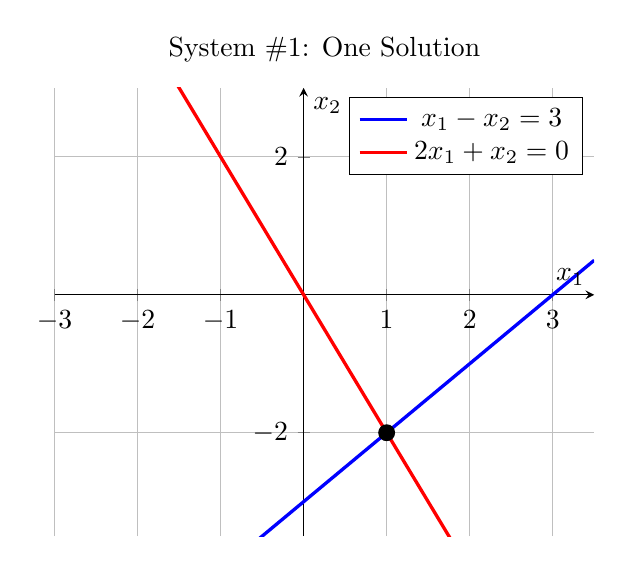
\begin{tikzpicture}[scale=\scl]
            \begin{axis}[axis lines=center, title={System \#1: One Solution}, domain=-3:3.5,
                xmin=-3, xmax=3.5, ymin=-3.5, ymax=3, xlabel={$x_1$}, ylabel={$x_2$}, grid]
                \addplot[very thick, blue, smooth] {(3-x)/(-1)};
                \addlegendentry{$x_1-x_2=3$};
                \addplot[very thick, red, smooth] {-2*x};
                \addlegendentry{$2x_1+x_2=0$};
                \draw[fill=black] (axis cs:1,-2) circle(0.1cm);
            \end{axis}
        \end{tikzpicture}
        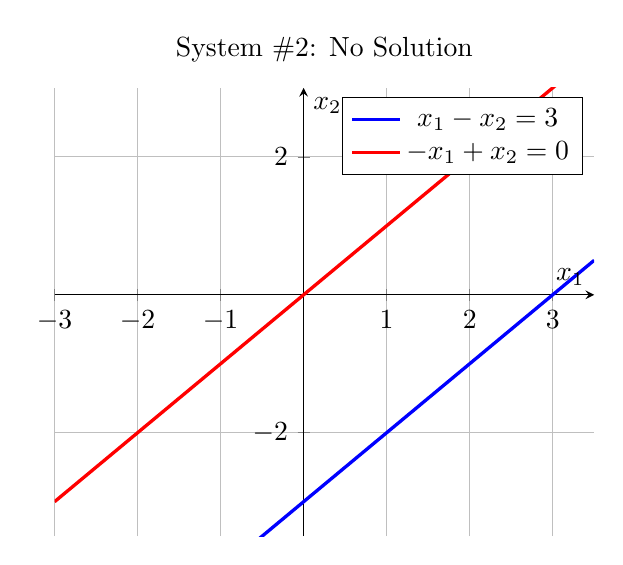
\begin{tikzpicture}[scale=\scl]
            \begin{axis}[axis lines=center, title={System \#2: No Solution}, domain=-3:3.5,
                xmin=-3, xmax=3.5, ymin=-3.5, ymax=3, xlabel={$x_1$}, ylabel={$x_2$}, grid]
                \addplot[very thick, blue, smooth] {(3-x)/(-1)};
                \addlegendentry{$x_1-x_2=3$};
                \addplot[very thick, red, smooth] {x};
                \addlegendentry{$-x_1+x_2=0$};
            \end{axis}
        \end{tikzpicture}
        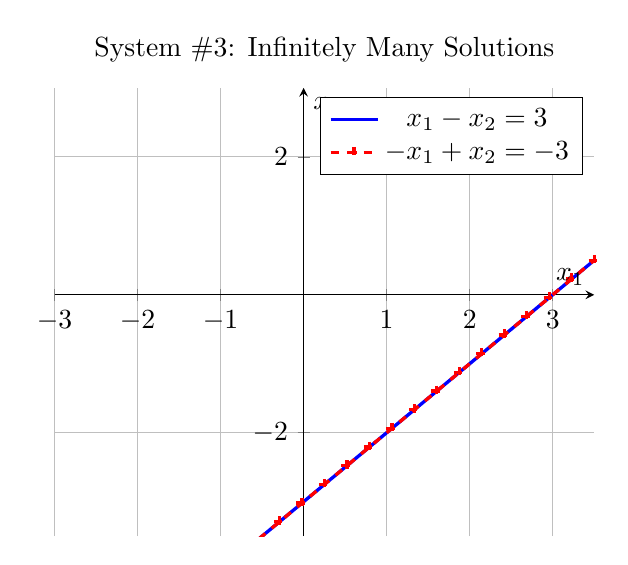
\begin{tikzpicture}[scale=\scl]
            \begin{axis}[axis lines=center, title={System \#3: Infinitely Many Solutions},
                    domain=-3:3.5, xmin=-3, xmax=3.5, ymin=-3.5, ymax=3, xlabel={$x_1$},
                ylabel={$x_2$}, grid]
                \addplot[very thick, blue, smooth] {(3-x)/(-1)};
                \addlegendentry{$x_1-x_2=3$};
                \addplot[very thick, red, dashed, mark=+] {(-3+x)};
                \addlegendentry{$-x_1+x_2=-3$};
            \end{axis}
        \end{tikzpicture}
    \end{center}
    \caption{Three possible solution sets in two spatial dimensions}
    \label{fig:10.3.soln_sets}
\end{figure}


\begin{example}
Solve the system of equations.  If there are infinitely many solution, express them as a
parameterization.
\begin{flalign*}
    -4x_1 + x_2 &= 0 \\
    -12 x_1 + 3x_2 &= 0
\end{flalign*}
{\bf Solution:}
First we write the system of equations as an augmented system.  Then we row reduce as much
as possible.
\begin{flalign*}
    \left( \begin{array}{cc|c} -4 & 1 & 0 \\ -12 & 3 & 0 \end{array} \right) &
        \stackrel{(-3)R_1 + R_2}{\longrightarrow}
    \left( \begin{array}{cc|c} -4 & 1 & 0 \\ 0 & 0 & 0 \end{array} \right) 
\end{flalign*}
In this particularly simple example, this means that $-4x_1 + 1x_2 = 0$.  Written another
way, $x_2 = 4x_1$. 

If we write $x_1 = t$ then the solution is $x_1=t, \, x_2 = 4t \text{ for } -\infty
< t < \infty$. If, on the other hand, we write $x_2 = t$ then the solution is
$x_2=t, \, x_1 = t/4 \text{ for } -\infty < t < \infty$.

In vector form, this solution can be written as
\[ \bpm x_1 \\ x_2 \epm = \bpm 1 \\ 4 \epm t \]
or
\[ \bpm x_1 \\ x_2 \epm = \bpm \frac{1}{4} \\ 1 \epm t. \]
\end{example}


\begin{example}
    Solve the system of equations $A\texttt{x} = \texttt{b}$ where
\[ A = \bpm 3 & 5 & -4 \\ -3 & -2 & 4 \\ 6 & 1 & -8 \end{pmatrix} \quad \text{and} \quad
    \texttt{b} = \bpm 7 \\ -1 \\ -4 \epm. \]
    {\bf Solution:} 
    Writing the augmented matrix $(A | \texttt{b})$ and doing several steps of row reduction gives
\[ \left( \begin{array}{ccc|c}
        3 & 5 & -4 & 7 \\
        -3 & -2 & 4 & -1 \\
        6 & 1 & -8 & -4 \end{array} \right)
    \longrightarrow 
    \left( \begin{array}{ccc|c}
        1 & 0 & -\frac{4}{3} & -1 \\
        0 & 1 & 0 & 2 \\
        0 & 0 & 0 & 0 \end{array} \right)
        \]

This implies that $x_2 = 2$ and $x_1 = -1 + \frac{4}{3} t$ for some parameter $t$.

Written in vector form, the solution is
\[ \bpm x_1 \\ x_2 \\ x_3 \epm = \bpm -1 \\ 2 \\ 0 \epm + t \bpm \frac{4}{3} \\ 0 \\ 1
    \epm. \]
\end{example}


\begin{example}
Solve the system of equations
\begin{flalign*}
    4x_1 + x_2 + 5x_3 + 7x_4 &= 0 \\
    8x_1 + x_2 - 5x_3 + 4x_4 &= 0
\end{flalign*}
{\bf Solution:} 
Written in augmented form and row reduced we see that 
\[ \left( \begin{array}{cccc|c}
        4 & 1 & 5 & 7 & 0 \\
        8 & 1 & -5 & 4 & 0 \end{array} \right)
        \longrightarrow
    \left( \begin{array}{cccc|c}
        4 & 1 & 5 & 7 & 0 \\
        0 & -1 & -15 & -10 & 0
    \end{array} \right) 
    \longrightarrow
    \left( \begin{array}{cccc|c}
        4 & 0 & -10 & -11 & 0 \\
        0 & 1 & 15 & 10 & 0 \end{array} \right)
    \]
In this case there are two variables that cannot be solve for: $x_3$ and $x_4$.  These are
now both parameters.  If $x_3 = s$ and $x_4 = t$ then
\[ x_1 = \frac{10s + 11t}{4} \quad \text{and} \quad x_2 = -15s - 10t \quad \text{where} \quad x_3=s
    \quad \text{and} \quad x_4 = t. \]

In vector form, this solution can be written as
\[ \bpm x_1 \\ x_2 \\ x_3 \\ x_4 \epm = \bpm 10/4 \\ -15 \\ 1 \\ 0 \epm s + \bpm 11/4 \\ -10
    \\ 0 \\ 1 \epm t. \]
\end{example}

% \input{activities/10.3.Act1b}
\begin{problem}
    Each of the following systems has been row reduced as much as possible.  If there is a
    unique solution to the system then find it.  If there are infinitely many solutions
    then express them as a vector equation.  If there are no solutions then indicate the
    reason.
    \begin{flalign}
        \left( \begin{array}{cccc|c} 
            1 & 2 & 0 & 0 & 3 \\ 
            0 & 0 & 1 & 0 & -2 \\ 
            0 & 0 & 0 & 0 & 0 \end{array} \right) \\
%
        \left( \begin{array}{cccc|c} 
            1 & 2 & 0 & 0 & 3 \\ 
            0 & 0 & 1 & 0 & -2 \\ 
            0 & 0 & 0 & 0 & 3 \end{array} \right) \\
%
        \left( \begin{array}{ccc|c} 
            1 & 0 & 2 & 3 \\ 
            0 & 1 & -1 & -2 \\ 
            0 & 0 & 0 & 0 \end{array} \right) \\
%
        \left( \begin{array}{ccc|c} 
            1 & 0 & 2 & 3 \\ 
            0 & 1 & 0 & -2 \\ 
            0 & 0 & 0 & 0 \end{array} \right) 
    \end{flalign}

\end{problem}


\newpage\section{Linear Combinations}
One of the most beautiful parts of linear algebra is the richness of the structure of
matrices.  As we showed earlier, every system of linear equations can be written several
different ways (as a system, as a matrix equation, as a vector equation, or as an
augmented system).  In this subsection we'll look in particular at the vector equation.
Hiding below a vector equation is one of the most fundamental ideas behind all of linear
algebra: the linear combination.

\begin{definition}
    Let $\texttt{v}_1, \texttt{v}_2, \ldots, \texttt{v}_p$ be vectors in $n$-dimensional space and let
    $c_1, c_2, \dots, c_p$ be scalar quantities.  The vector $\texttt{u}$ defined by
    \[ \texttt{u} = c_1 \texttt{v}_1 + c_2 \texttt{v}_2 + \cdots c_p \texttt{v}_p \]
    is called a {\bf linear combination} of the vectors $\texttt{v}_1, \texttt{v}_2, \dots,
    \texttt{v}_p$ with weights $c_1, c_2, \dots, c_p$.
\end{definition}

In the system of equations
\begin{flalign}
    2x_1 + 3x_2 &= 5 \\
    4x_1 - 6x_2 &= 6,
\end{flalign}
we can rephrase the underlying question as: {\it find the weights which solve the vector
equation}
\begin{flalign}
    x_1 \bpm 2 \\ 4 \epm + x_2 \bpm 3 \\ -6 \epm = \bpm 5 \\ 6 \epm.
    \label{eqn:10.3.lincom}
\end{flalign}
Notice that this is simply stating that a system of equations is nothing more than a
linear combination with unknown weights!

There is also a nice graphical interpretation of linear combination
\eqref{eqn:10.3.lincom}: How many $\bpm 2\\4\epm$ plus how many $\bpm 3\\-6\epm$ do we
need to create $\bpm5\\6\epm$? Solving for $x_1$ and $x_2$ (using Gaussian elimination) we
find that $x_1=2$ and $x_2 = 1/3$.  Hence, {\color{black} $\bpm5\\6\epm =$} {\color{red}
$2\bpm2\\4\epm$} $+$ {\color{blue} $(1/3)\bpm3\\-6\epm$} as seen in Figure
\ref{fig:10.3.lincom}.
\begin{figure}[ht!]
    \begin{center}
        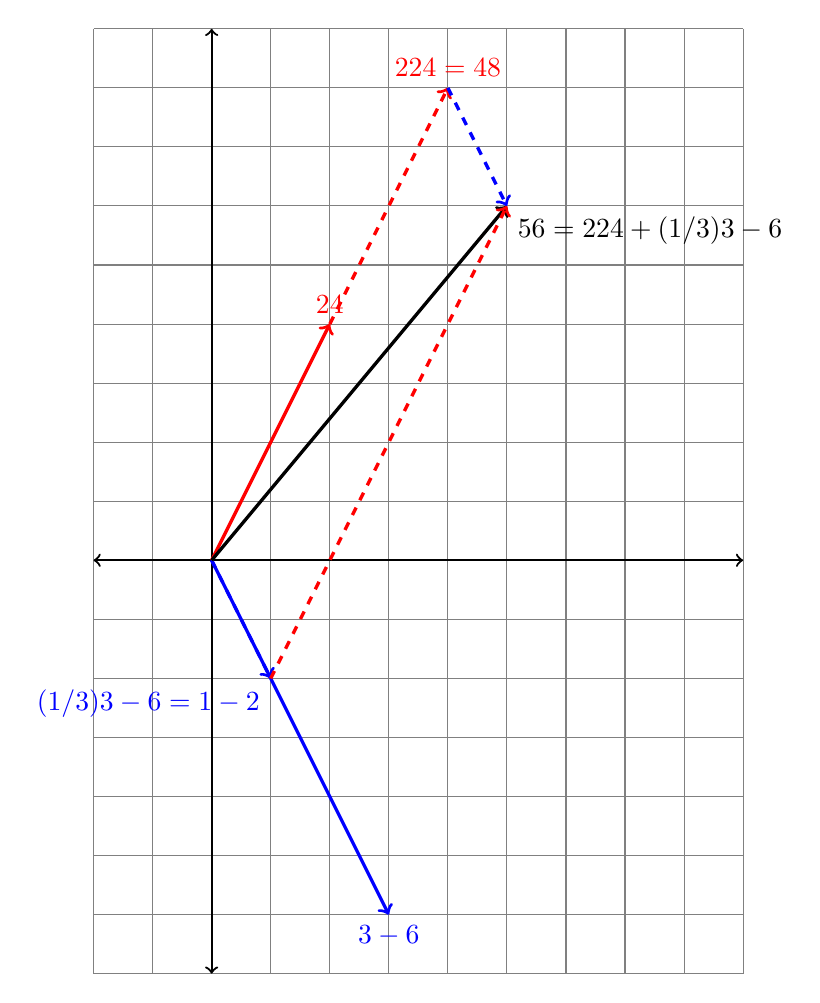
\begin{tikzpicture}[scale=0.75]
            \draw[gray] (-2,-7) grid (9,9);
            \draw[<->,thick, black] (-2,0) -- (9,0);
            \draw[<->,thick, black] (0,-7) -- (0,9);
            \draw[red, very thick,->] (0,0) -- (2,4) node[anchor=south]{$\bpm2\\4\epm$};
            \draw[red, very thick, dashed,->] (2,4) -- (4,8)
            node[anchor=south]{$2\bpm2\\4\epm=\bpm4\\8\epm$};
            \draw[blue, very thick,->] (0,0) -- (3,-6) node[anchor=north]{$\bpm3\\-6\epm$};
            \draw[blue, very thick, dashed,->] (0,0) -- (1,-2) node[anchor=north east]{$(1/3)\bpm3\\-6\epm=\bpm1\\-2\epm$};
            \draw[black, very thick,->] (0,0) -- (5,6) node[anchor=north
            west]{$\bpm5\\6\epm=2\bpm2\\4\epm + (1/3)\bpm3\\-6\epm$};
            \draw[red, very thick, dashed, ->] (1,-2) -- (5,6);
            \draw[blue, very thick, dashed,->] (4,8) -- (5,6);
        \end{tikzpicture}
    \end{center}
    \caption{A graphical example of a linear combination.}
    \label{fig:10.3.lincom}
\end{figure}

% \input{activities/10.3.Act2}
\begin{problem}
    Open the GeoGebra applet
    \href{http://tube.geogebra.org/student/m1254137}{http://tube.geogebra.org/student/m1254137} in a browser window.
    \ba
        \item Move the vectors $\bu$ and $\bv$ to 
            \[ \bu = \bpm 1 \\ 2 \epm \quad \text{and} \quad \bv = \bpm 2 \\ -1 \epm. \]
            We would like to determine all of the combinations possible forming the vector
            \[ \bw = c_1 \bu + c_2 \bv. \]
            Use the sliders in the GeoGebra applet to answer the following questions:
            \begin{enumerate}
                \item[(i)] Describe all of the possible vectors $\bw$ if $c_1=0$.
                \item[(ii)] Describe all of the possible vectors $\bw$ if $c_2=0$.
                \item[(iii)] Which vector results if $c_1=c_2=0$?
                \item[(iv)] Is it possible to find $c_1$ and $c_2$ such that $\bw = \bpm
                    -6 \\ 0.5 \epm$?  If so, what are $c_1$ and $c_2$.  If not, why not?
            \end{enumerate}
        \item Move $\bu$ and $\bv$ so they are parallel.  Form the vector $\bw = c_1 \bu +
            c_2 \bv$ and describe all of the possible values of the vector $\bw$.
        \item Find $c_1$ and $c_2$ both algebraically and graphically so that
            \[ \bpm 1 \\ -12 \epm = c_1 \bpm 1 \\ -2 \epm + c_1 \bpm 0 \\ 2 \epm. \]

        \item Express the vector $\bw = \bpm 5 \\ -4 \epm$ as a linear comination of $\bu =
    \bpm -2 \\ -1 \epm$ and $\bv = \bpm 1 \\ -6 \epm$.  
    \ea

\end{problem}




\newpage\section{Inverses and Determinants} \label{S:10.4.InvDet}
Division is always a bit of a touchy subject.  In the real numbers division is well
defined except when the denominator is zero.  The same story is true in the rational
numbers: a fraction divided by a fraction is another fraction so long as the divisor is
not zero.  What if we wanted to stay only in the integers?  Can we divide two integers and
get another integer?  Of course you can always divide by 1, but in most other cases
division will move you into the rational numbers.  Hence, division on the integers doesn't
really make sense.\footnote{The mathematician would say that the integers are not closed
under division.} 

Similarly, if we try to define division on matrices we run into trouble.  What does it
mean to {\it divide by a matrix}?  In general, that phrase is meaningless!  Let's expand
our view a bit.

When considering the operation of addition, we call $0$ the {\bf additive identity} and we
call $(-a)$ the {\it additive inverse} of $a$ since $a + (-a) = 0$.  When considering
multiplication, we call $1$ the {\bf multiplicative identity} and $1/a$ is the {\it
multiplicative inverse} of $a$ (when $a \ne 0$) since $a \cdot \frac{1}{a} = 1$.  



% \input{previews/10.4.PA1}
\begin{problem}
    Consider the matrix
    \[ A = \bpm 1 & 2 \\ -4 & 3 \epm. \]
    \ba
        \item Find a matrix $B$ such that $A + B = A$ and $B + A  = A$.
        \item Find a matrix $I$ such that $I \cdot A = A$ and $A \cdot I = A$.
        \item Find a matrix $C$ such that $C \cdot A = I$ and $A \cdot C = I$.
    \ea
\end{problem}

One way to tackle the third part of the preceding problem is let let $C$ be a
matrix filled with unknowns and then to build the associated system of equations.  More
specifically, if we let 
\[ C = \begin{pmatrix} a & b \\ c & d \end{pmatrix} \]
and then observe that the equation $AC = I$ becomes
\[ \begin{pmatrix} 1 & 2 \\ -4 & 3 \end{pmatrix} \begin{pmatrix} a & b \\ c & d
\end{pmatrix} = \begin{pmatrix} 1 & 0 \\ 0 & 1 \end{pmatrix}. \]
After multiplying the left-hand side we get the equation
\[ \begin{pmatrix} a + 2c & b + 2d \\ -4a + 3c & -4b + 3d \end{pmatrix} = \begin{pmatrix}
    1 & 0 \\ 0 & 1 \end{pmatrix}. \]
This results in a system of four equations with four unknowns:
\[ \left\{ \begin{array}{rl} a + 2c &= 1 \\ b+2d &= 0 \\ -4a + 3c &= 0 \\ -4b + 3d &= 1
\end{array} \right. \]
which can be solved using Gaussian Elimination (row reduction):  
\[ \left( \begin{array}{cccc|c} 1 & 0 & 2 & 0 & 1 \\
        0 & 1 & 0 & 2 & 0 \\
        -4 & 0 & 3 & 0 & 0 \\
    0 & -4 & 0 & 3 & 1 \end{array} \right) \to \cdots \to 
\left( \begin{array}{cccc|c} 1 & 0 & 0 & 0 & 3/11 \\
    0 & 1 & 0 & 0 & -2/11 \\
    0 & 0 & 1 & 0 & 4/11 \\
    0 & 0 & 0 & 1 & 1/11 \end{array} \right).
    \]
Hence, 
\[ C = \frac{1}{11} \begin{pmatrix} 3 & -2 \\ 4 & 1 \end{pmatrix}. \]
You should fill in all of the missing row reduction to verify this answer.  Also, to check
this answer you should multiply $AC$ and $CA$ to be sure that you get the identity matrix
with both multiplications.

\begin{definition}
    In matrices we define the following:
    \begin{itemize}
        \item The {\bf additive identity} of an $m \times n$ matrix is
            \[ 0_{m\times n} = \bpm 0 & 0 & \cdots & 0 \\ 0 & 0 & \vdots & \vdots \\
            \vdots & \vdots & \ddots & \vdots \\ 0 & 0 & \cdots & 0 \epm. \]
        \item The {\bf additive inverse} of an $m \times n$ matrix $A$ is $(-A)$ since $A
            + (-A) = (-A) + A = 0$.
        \item The {\bf multiplicative identity} of an $n\times n$ matrix $A$ is the matrix 
            \[ I = \bpm 1 & 0 & 0 &\cdots & 0 \\ 
                        0 & 1 & 0 & \cdots & 0 \\
                        0 & 0 & \ddots &  & \vdots \\
                        \vdots & \vdots &  & \ddots & 0 \\
                        0 & 0 & \cdots & 0 & 1 \epm \]
        \item The {\bf multiplicative inverse} of an $n \times n$ matrix $A$ is an $n
            \times n$ matrix $C$ such that $AC = CA = I$.
    \end{itemize}
\end{definition}
The zero matrix act's like the zero integer; adding the zero matrix doesn't change the
sum.  Similarly, the identity matrix (with ones down the main diagonal and zeros
elsewhere) acts like the integer 1; when multiplying by the identity matrix the product
doesn't change.

\subsection{Inverses}
The following activity defines the matrix inverse for a $2\times 2$ matrix.  The reader
should carefully work this problem and take careful note of the result since it shows the
general process for finding inverses.

% \input{activities/10.4.Act1}
\begin{problem}
    Consider the matrix $A = \bpm 2 & 3 \\ 2 & 4 \epm$. We would like to find the inverse
    of $A$ so that when we multiply the inverse by $A$ we get the identity $I$.
    \ba
        \item Let's first try a na\:ive {\it inverse}.  Let 
            \[ B = \bpm 1/2 & 1/3 \\ 1/2 & 1/4 \epm. \]
            Find the products $AB$ and $BA$ and verify that $AB \neq I$ and $BA \neq I$.
            
            We really want to find the matrix $B$ such that $AB = BA = I = \bpm 1 & 0 \\ 0
            & 1 \epm$.  The following parts of this activity will guide you toward that
            goal.
        \item Create an augmented matrix $(A \, | \, I)$.
        \item Use elementary row operations to reduce the matrix in part (a) to an
            augmented matrix of the form $(I \, | \star)$.
        \item Check that the matrix on the right-hand side of your answer in part (b) is
            actually the inverse of $A$.
        \item Now consider the matrix $A = \bpm a & b \\ c & d \epm$.  Repeat parts (a)
            and (b) to find the inverse of a general $2 \times 2$ matrix.  You should have
            a factor of $\frac{1}{ad-cb}$ in your matrix.  The denominator of this
            fraction is called the {\it determinant} of the matrix $A$.
    \ea

\end{problem}

The previous problem illustrated the method for finding the inverse of a matrix:
\begin{technique}[Process for finding $A^{-1}$ if it exists]
    The following is the technique for find the inverse of a matrix (if it exists).
    \begin{enumerate}
        \item augment the matrix with the identity, then
        \item row reduce to get the identity on the left-hand side of the augmented matrix.
    \end{enumerate}
\end{technique}

\begin{example}
Let's find the inverse of the matrix from the preview activity using this method instead.
Let $A = \begin{pmatrix} 1 & 2 \\ -4 & 3 \end{pmatrix}$.  We want to find $A^{-1}$ such
that $AA^{-1} = I$ and $A^{-1} A = I$. 
\\{\bf Solution:}
Using the equation $AA^{-1} = I$ and knowing that we are seeking $A^{-1}$ we can write the
augmented system $\left( A \, | \, I \right)$ and row reduce until we get $\left( I \, |
\, A^{-1} \right)$: 
\begin{flalign*}
    \left( A \, | \, I \right) &= \left( \begin{array}{cc|cc} 1 & 2 & 1 & 0 \\ -4 & 3 & 0
        & 1 \end{array} \right)  \\
    &\to \left( \begin{array}{cc|cc} 1 & 2 & 1 & 0 \\ 0 & 11 & 4 & 1 \end{array} \right)  \\
    &\to \left( \begin{array}{cc|cc} 1 & 2 & 1 & 0 \\ 0 & 1 & 4/11 & 1/11 \end{array} \right)  \\
    &\to \left( \begin{array}{cc|cc} 1 & 0 & 3/11 & -2/11 \\ 0 & 1 & 4/11 & 1/11
    \end{array} \right) = \left( I \, | \, A^{-1} \right)  \\
\end{flalign*}
Hence, the inverse of $A$ is $A^{-1} = \frac{1}{11} \begin{pmatrix} 3 & -2 \\ 4 & 1
\end{pmatrix}$
\end{example}

\begin{example}
In part (e) of the previous activity you also worked to find the inverse for the generic
$2 \times 2$ matrix $A = \begin{pmatrix} a & b \\ c & d \end{pmatrix}$.  If you did all of
your work correctly you will have found that 
\[ A^{-1} = \frac{1}{ad-bc} \cdot \begin{pmatrix} d & -b \\ -c & a \end{pmatrix}. \]
Let's use this formula to verify (for a third time) the inverse of the matrix from the
preview.
\\{\bf Solution:}
Since $A = \begin{pmatrix} 1 & 2 \\ -4 & 3 \end{pmatrix}$ we can apply the $2 \times 2$
inverse formula to get
\[ A^{-1} = \frac{1}{(1)(3) - (2)(-4)} \cdot \begin{pmatrix} 3 & -2 \\ 4 & 1 \end{pmatrix}
= \frac{1}{11} \begin{pmatrix} 3 & -2 \\ 4 & 1 \end{pmatrix} \]
\end{example}
The reader should be cautious here.  The formula that you derived for $2 \times 2$
matrices only makes sense for that size.  The only true method for finding the inverse
(with the tools we have) is to augment your matrix with the identity and to row reduce.

One other trouble comes when it is impossible to get the identity matrix to appear on the right.
When this happens it is an indication that the matrix does not have a multiplicative
inverse.  In the following activity you will practice this technique on a few matrices.
% 
% \input{activities/10.4.Act2}
\begin{problem}
    Find the inverse for each of the following matrices if it exists.  If it does not
    exist then determine why not.
    \ba
        \item $\bpm 1 & -3 \\ 4 & -9 \epm$
        \item $\bpm 3 & 6 \\ 4 & 7 \epm$
        \item $\bpm 1 & 2 & -1 \\ -4 & -7 & 3 \\ -2 & -6 & 4 \epm$
        \item $\bpm 1 & 0 & 0 \\ 1 & 1 & 0 \\ 1 & 1 & 1 \epm$
    \ea

\end{problem}

\subsection{Determinants}
Finding a matrix inverse is often a tedious task.  As it turns out, there is a
very handy number associated with a square matrix that one can use to determine if a
matrix is invertible\footnote{This is actually one of many tests that you can be used to
determine if a matrix is invertible. A discussion of such techniques will wait until you
know a bit more linear algebra.}.  As we saw previously, if the
quantity $ad-bc$ is zero in the $2 \times 2$ matrix $\bpm a & b \\ c & d \epm$ then the
matrix cannot have an inverse.  This is not a peculiarity of $2 \times 2$ matrices!  The
value $ad-bd$ is called the determinant of the $2 \times 2$ matrix.  

What we need is a way to define the {\bf determinant} of a square matrix of any size.  In
order to do so it is easiest to observe how the formula works by following a pattern rather
than reading the technical definition.  The next problem will walk you through the
process.

% \input{activities/10.4.Act3}
\begin{problem}
    Follow these instructions to see how to find a determinant of a square matrix.
    \ba
        \item Find the determinant of the $2 \times 2$ matrix $\bpm 4 & -1 \\ -2 & 1 \epm$
            using the fact that 
            \[ \det(A) = \det \bpm a & b \\ c & d \epm = \left| \begin{array}{cc} a & b \\
                c & d \end{array} \right| = ad - bc. \]
        \item Now consider the matrix 
            \[ A = \bpm 1 & 5 & 3 \\ 2 & 4 & -1 \\ 0 & -2 & 0 \epm. \]
            \begin{itemize}
                \item[(i)] Cross out row 1 and column 1.  Call the resulting $2 \times 2$
                    matrix $A_{11}$.
                \item[(ii)] Cross out row 1 and column 2.  Call the resulting $2 \times 2$
                    matrix $A_{12}$.
                \item[(iii)] Cross out row 1 and column 3.  Call the resulting $2 \times 2$
                    matrix $A_{13}$.
                \item[(iv)] The determinant of $A$ is
                    \[ \det(A) = 1 \cdot \det(A_{11}) - 5 \cdot \det(A_{12}) + 3 \cdot
                    \det(A_{13}). \]
                    Perform this computation.
            \end{itemize}

        \item Find the determinant of the matrix 
            \[ A = \bpm 2 & 3 & -4 \\ 4 & 0 & 5 \\ 5 & 1 & 6 \epm. \]

        \item Fill in the blanks below to set up the determinant calculation for the
            following $4 \times 4$ matrix.
            \[ A = \bpm 2 & 3 & 5 & 7 \\
                        0 & 3 & 2 & 9 \\
                        3 & -2 & 6 & 1 \\
                        2 & 0 & 0 & 4 \epm \]
            \[ \det(A) = 2 \cdot \left| \begin{array}{ccc} 
                    \underline{\hspace{0.2in}} & \underline{\hspace{0.2in}} & \underline{\hspace{0.2in}} \\
                    \underline{\hspace{0.2in}} & \underline{\hspace{0.2in}} & \underline{\hspace{0.2in}} \\
                    \underline{\hspace{0.2in}} & \underline{\hspace{0.2in}} & \underline{\hspace{0.2in}} 
                \end{array} \right| 
                - 3 \cdot \left| \begin{array}{ccc} 
                    \underline{\hspace{0.2in}} & \underline{\hspace{0.2in}} & \underline{\hspace{0.2in}} \\
                    \underline{\hspace{0.2in}} & \underline{\hspace{0.2in}} & \underline{\hspace{0.2in}} \\
                    \underline{\hspace{0.2in}} & \underline{\hspace{0.2in}} & \underline{\hspace{0.2in}} 
                \end{array} \right|
                + 5 \cdot \left| \begin{array}{ccc} 
                    \underline{\hspace{0.2in}} & \underline{\hspace{0.2in}} & \underline{\hspace{0.2in}} \\
                    \underline{\hspace{0.2in}} & \underline{\hspace{0.2in}} & \underline{\hspace{0.2in}} \\
                    \underline{\hspace{0.2in}} & \underline{\hspace{0.2in}} & \underline{\hspace{0.2in}} 
                \end{array} \right|
                -7\cdot \left| \begin{array}{ccc} 
                    \underline{\hspace{0.2in}} & \underline{\hspace{0.2in}} & \underline{\hspace{0.2in}} \\
                    \underline{\hspace{0.2in}} & \underline{\hspace{0.2in}} & \underline{\hspace{0.2in}} \\
                    \underline{\hspace{0.2in}} & \underline{\hspace{0.2in}} & \underline{\hspace{0.2in}} 
                \end{array} \right|
                \]

            \item In your notes, write a few sentences describing the process for finding
                determinants of square matrices.
    \ea

\end{problem}

\begin{example}
In this example we will work through the determinant of the $3 \times 3$ matrix 
\[ A = \begin{pmatrix} 1 & 0 & 3 \\ 
                       0 & 2 & -5 \\ 
                       0 & 0 & 3 \end{pmatrix} \]
{\bf Solution:} 
Let's expand along the first row:
\begin{flalign*}
    \det(A) &= 1 \cdot \left| \begin{array}{cc} 2 & -5 \\ 0 & 3 \end{array} \right| - 0
    \cdot \left| \begin{array}{cc} 0 & -5 \\ 0 & 3 \end{array} \right| + 3 \cdot \left|
    \begin{array}{cc} 0 & 2 \\ 0 & 0 \end{array} \right| \\
    &= 1 \cdot \left( (2)(3) - (0)(-5) \right) - 0 \cdot \left( (0)(3) - (0)(-5) \right) +
    3 \cdot \left( (0)(0) - (0)(2) \right) \\
    &= 1 \cdot 6 - 0 \cdot 0 + 3 \cdot 0 \\
    &= 6.
\end{flalign*}
Also notice in this example that the entire lower triangle of the matrix is filled with
zeros.  When this is the case you may observe the nice pattern that the determinant is
actually just the product of the entries on the main diagonal (you should prove that this
is true).  Hence, in this problem we know that $\det(A) = 1 \cdot 2 \cdot 3 = 6$.  Be
careful!  If you don't have an entire triangle of zeros then this little {\it trick} will
not work.
\end{example}

\begin{problem}
    Find the determinant of the following matrices.  Is there anything special that you
    can say about these matrices?  Do you notice any ways to make the determinant
    computation faster on these matrices?
    \begin{flalign*}
        A &= \begin{pmatrix} 1 & 3 \\ 6 & 2 \end{pmatrix} \\
        B &= \begin{pmatrix} 1 & 3 \\ 2 & 6 \end{pmatrix} \\
        C &= \begin{pmatrix} 2 & 3 & 2 \\ 4 & 7 & 3 \\ 1 & 0 & 5 \end{pmatrix} \\
        D &= \begin{pmatrix} 2 & 3 & 2 \\ 0 & 0 & 3 \\ 1 & 0 & 5 \end{pmatrix} \\
        E &= \begin{pmatrix} 2 & 3 & 2 \\ 0 & 7 & 3 \\ 0 & 0 & 5 \end{pmatrix}
    \end{flalign*}
\end{problem}


\begin{problem}
    Find the value of $k$ so that the matrix $A$ is not invertible.
    \[ A = \begin{pmatrix} 2 & 4 \\ 3 & k \end{pmatrix} \]
\end{problem}

\begin{problem}
    Given the matrix 
    \[ B = \begin{pmatrix} 2-x & 1 \\ 4 & 2-x \end{pmatrix} \]
    find all of the values of $x$ that are solutions to the equation $\det(B) = 0$.
\end{problem}


The following Theorem states several properties of determinants.  While these are all very
useful in their own right, we will not take the time here to expand upon their proofs.

\begin{thm}[Important Properties of Determinants]\label{thm:10.4.det}
    Let $A$ be a square matrix.
    \begin{enumerate}
        \item The determinant of the identity matrix is 1.
        \item The $n \times n$ matrix $A$ is invertible if and only if $\det(A) \ne 0$
        \item $\det(A^T) = \det(A)$.
        \item $\det(AB) = \det(A) \det(B)$
        \item $\det(A^{-1}) = 1/\det(A)$
        \item If $A$ is an $n \times n$ matrix and $c$ is a real number then
            $\det(c A) = c^n \det(A)$ 
        \item If a multiple of one row of $A$ is added to another row to produce matrix
            $B$ then $\det(A) = \det(B)$.
        \item If two rows are interchanged in matrix $A$ to produce matrix $B$ then
            $\det(B) = -\det(A)$.
        \item If one row of $A$ is multiplied by $k$ to product matrix $B$ then $\det(B) =
            k \det(A)$.
        \item The absolute value of the determinant of a matrix $A$ is the volume of the parallelepiped
            formed by the column vectors of $A$. (In 2D this means that the determinant is
            the area of the associated parallelogram.)
    \end{enumerate}
\end{thm}

In Theorem \ref{thm:10.4.det}, every property listed has significant impact on the
computation of determinants and inverses. The final activity in this section illustrated
the time savings and possible pitfalls that can occur.

% \input{activities/10.4.Act4}
\begin{problem}
    In this activity we'll explore a few properties of the determinant.
    \ba
        \item How do $\det(A)$ and $\det(A^{-1})$ relate to each other? Hint: we know that
            $AA^{-1} = I$.
        \item Determine if the matrix $B$ is invertible without trying to calculate the
            inverse.
            \[ B = \bpm 2 & 4 & -3 \\ 0 & 0 & 7 \\ 0 & 0 & 3 \epm \]
        \item If the entries in a $10 \times 10$ matrix $A$ are known to within a 5\%
            error, what is the maximum error in the determinant computation? \\ Hint: Let
            $c=1.05$.  What is $\det(cA)$?
    \ea
\end{problem}
% 
The last problem in the previous problem should serve as a warning!  When doing a
determinant computation on a computer there is natural roundoff error due to the fact that
any number stored in a computer can only be stored with finite bits.  Hence, every
determinant computation on a large matrix should be immediately suspect! For this reason,
it is often preferred to avoid the use of the determinant if at all possible when dealing
with large matrices. 

\begin{problem}
    If $A = \begin{pmatrix} a & b \\ c & d \end{pmatrix}$ and $\det(A) = 8$ then what is
        $\det(B)$ where $B = \begin{pmatrix} a & b \\ 3c & 3d \end{pmatrix}$
\end{problem}
\solution{$\det(B) = 3\cdot8 = 24$}


\begin{problem}
    If $A = \begin{pmatrix} a & b \\ c & d \end{pmatrix}$ and $\det(A) = 8$ then what is
    $\det(B)$ where $B = \begin{pmatrix} a & b \\ 2a+c & 2b + d \end{pmatrix}$    
\end{problem}
\solution{24}


\begin{problem}
    True or False: The determinant of $A$ is the same as the determinant of the row
    reduced form of $A$.  Explain your answer.
\end{problem}
\solution{False.  Row reduction often leads swapping and scaling rows}


The last statement of Theorem \ref{thm:10.4.det} give a bit of a deeper insight
to the geometry of determinants and why invertible matrices must have a non-zero
determinant.  Think about a $2 \times 2$ matrix with non-zero determinant.  Under matrix
multiplication by this matrix, a shape with non-zero area will be transformed to another
shape with non-zero area.  Hence, if we were to reverse the mapping then we have all of
the vectors accounted for and can reverse the transformation.  If, on the other hand, a
matrix has a determinant of zero then a shape with non-zero area will be transformed into
a shape with zero area.  Naturally, in this case, many vectors will be mapped on top of
each other and any hope of reversing the transformation is lost -- hence the fact that a
matrix with a zero determinant is not invertible.

For example, if we consider the matrix $A = \begin{pmatrix} 2&1\\1&2\end{pmatrix}$, the
determinant is $\det(A) = 4-1=3 \ne 0$ and we know that $A^{-1}$ exists.  To see the
action on the vectors $\bu_1 = \begin{pmatrix}1\\0\end{pmatrix}$ and $\bu_2 =
\begin{pmatrix}0\\1\end{pmatrix}$ see Figure \ref{fig:determinant_vol_1}.  Notice that
before the multiplication by $A$ the parallelogram (square) formed by $\bu_1$ and $\bu_2$ is 1
(since the determinant of the identity is 1).  After the multiplication by $A$ the
original square is stretched into the parallelogram on the right of Figure
\ref{fig:determinant_vol_1} and with some geometry we can see that the area of the
parallelogram is $3$.  If we were to imagine reversing the transformation, morphing the
red parallelogram back into the blue square, we can see visually how each vector in the plane gets
stretched and rotated -- hence giving a good meaning to {\it reversing} the
transformation and giving us a visual sense that the inverse of $A$ exists.

Now consider the matrix $A = \begin{pmatrix}2&1\\1&0.5\end{pmatrix}$.  The determinant of
this matrix is clearly zero, and geometrically in Figure \ref{fig:determinant_vol_2} we
see that the square gets {\it squished} into a single line segment with zero area.  In
fact, both of the vectors $\bu_1$ and $\bu_2$ are mapped to exactly the same line segment
and figuring out how to reverse these actions for every vector in the plane is impossible
-- hence giving us a sense that if the determinant is zero then the inverse of the matrix
$A$ must not exist.

\begin{figure}[ht!]
    \begin{center}
        \begin{tikzpicture}
            \begin{axis}[axis lines=center, axis equal, grid, xmin=-1, xmax=3, ymin=-1,
                ymax=3, title={The vectors $\bu_1=\begin{pmatrix}1\\0\end{pmatrix}$ and
            $\bu_2 = \begin{pmatrix}0\\1\end{pmatrix}$}]
                \draw[fill=gray!50, opacity=0.3] (axis cs:0,0) -- (axis cs:1,0) -- (axis
                cs:1,1) -- (axis cs:0,1) -- (axis cs:0,0);
                \draw[very thick, blue, ->] (axis cs:0,0) -- (axis cs:1,0);
                \draw[very thick, blue, ->] (axis cs:0,0) -- (axis cs:0,1);
                \draw[very thick, dashed, blue, ->] (axis cs:1,0) -- (axis cs:1,0.95);
                \draw[very thick, dashed, blue, ->] (axis cs:0,1) -- (axis cs:0.95,1); 
            \end{axis}
        \end{tikzpicture}
        \begin{tikzpicture}
            \begin{axis}[axis lines=center, axis equal, grid, xmin=-1, xmax=3, ymin=-1,
                ymax=3, title={$A\bu_1=\begin{pmatrix}2\\1\end{pmatrix}$ and $A\bu_2=\begin{pmatrix}1\\2\end{pmatrix}$}]
                \draw[fill=red!50, opacity=0.3] (axis cs:0,0) -- (axis cs:2,1) -- (axis
                cs:3,3) -- (axis cs:1,2) -- (axis cs:0,0);
                \draw[very thick, red, ->] (axis cs:0,0) -- (axis cs:2,1);
                \draw[very thick, red, ->] (axis cs:0,0) -- (axis cs:1,2);
                \draw[very thick, dashed, red, ->] (axis cs:2,1) -- (axis cs:2.975,2.95);
                \draw[very thick, dashed, red, ->] (axis cs:1,2) -- (axis cs:2.95,2.975); 
            \end{axis}
        \end{tikzpicture}
    \end{center}
    \caption{A 2D mapping from region with non-zero area to a region non-zero area.}
    \label{fig:determinant_vol_1}
\end{figure}

\begin{figure}[ht!]
    \begin{center}
        \begin{tikzpicture}
            \begin{axis}[axis lines=center, axis equal, grid, xmin=-1, xmax=3, ymin=-1,
                ymax=3, title={The vectors $\bu_1=\begin{pmatrix}1\\0\end{pmatrix}$ and
            $\bu_2 = \begin{pmatrix}0\\1\end{pmatrix}$}]
                \draw[fill=gray!50, opacity=0.3] (axis cs:0,0) -- (axis cs:1,0) -- (axis
                cs:1,1) -- (axis cs:0,1) -- (axis cs:0,0);
                \draw[very thick, blue, ->] (axis cs:0,0) -- (axis cs:1,0);
                \draw[very thick, blue, ->] (axis cs:0,0) -- (axis cs:0,1);
                \draw[very thick, dashed, blue, ->] (axis cs:1,0) -- (axis cs:1,0.95);
                \draw[very thick, dashed, blue, ->] (axis cs:0,1) -- (axis cs:0.95,1); 
            \end{axis}
        \end{tikzpicture}
        \begin{tikzpicture}
            \begin{axis}[axis lines=center, axis equal, grid, xmin=-1, xmax=3, ymin=-1,
                ymax=3, title={$A\bu_1=\begin{pmatrix}2\\1\end{pmatrix}$ and
            $A\bu_2=\begin{pmatrix}1\\0.5\end{pmatrix}$}]
                \draw[very thick, red,->] (axis cs:0,0) -- (axis cs:2,1);
                \draw[very thick, red,->] (axis cs:0,0) -- (axis cs:1,0.5);
            \end{axis}
        \end{tikzpicture}
    \end{center}
    \caption{A 2D mapping from a region non-zero area to a region with zero area.}
    \label{fig:determinant_vol_2}
\end{figure}




\newpage\section{Technology For Linear Algebra}
There are many technological tools designed to efficiently perform linear algebra
operations.  At this stage in many student's academic careers they are very familiar with
the TI calculators (TI-89, TI-Nspire, TI-Voyage 200, etc).  The computer software MatLab
is also very prevalent in many colleges and industries as well as Maple, Mathematica,
Sage, MS Excel, and many many others.  The following is a very brief guide to using the TI
Calculator and MatLab for common operations. If the reader wants more information about
how to use these tools they are only an internet search away.

\begin{description}
    \item[Entering matrices:]  Consider the matrix $A = \bpm 1 & 2 & 3 \\ 4 & 5 & 6 \\ 7 &
        8 & 9 \epm$.
        \begin{description}
            \item[MatLab:] A matrix is written in square brackets with columns separated
                by commas and rows separated by semicolons.
\begin{verbatim}
A = [1 , 2 , 3 ; 4 , 5 , 6 ; 7 , 8 , 9]
\end{verbatim}
            \item[TI Calculator:] A matrix is written with curly brackets around the
                entire matrix and curly brackets around each row.  The rows and entries
                are separated by commas.
\begin{verbatim}
{{1,2,3},{4,5,6},{7,8,9}} -> A
\end{verbatim}
                The right arrow is the \texttt{STO} button.  Storing the matrix as a
                letter will allow you to do computations with the matrix.
        \end{description}

    \item[Arithmetic:] Addition, subtraction, and multiplication all work as expected in
        both pieces of software.
    \item[Transpose:] The transpose switches the rows and columns.
        \begin{description}
            \item[MatLab:] The apostrophe is the transpose operator in MatLab. For
                example, $B=A^T$ in MatLab is
\begin{verbatim}
B = [1 , 2 , 3 ; 4 , 5 , 6 ; 7 , 8 , 9]'
\end{verbatim}
            \item[TI Calculator:] After entering your matrix and storing it as a variable,
                the additional matrix operations are found under the \texttt{MATH} --
                \texttt{Matrix} menu.  The \texttt{MATH} menu is \texttt{2ND} --
                \texttt{5}.
        \end{description}
    \item[Reduced Row Echelon Form:] Both pieces of software will perform elementary row
        operations with the \texttt{rref} command.
    \item[Solving Systems in MatLab:] The \texttt{rref} command will give the reduced form
        of the matrix, but to solve a system, MatLab has a very powerful system solver:
        the \verb|\|.  As an example, consider the matrix equation
        \[ \bpm 1 & 2 & 3 \\ 4 & 5 & 6 \\ 7 & 8 & -2 \epm \bpm x_1 \\ x_2 \\ x_3 \epm =
        \bpm -3 \\ 2 \\ 7 \epm \quad \text{symbolically:} \quad A \texttt{x} =
    \texttt{b} \]
\begin{verbatim}
A = [1 , 2 , 3 ; 4 , 5 , 6 ; 7 , 8 , -2];
b = [-3 ; 2 ; 7];
x = A\b
\end{verbatim}
\end{description}


\newpage
% \section{Span, Linear Independence and Basis} \label{S:10.5.IndependenceDependenceBasis}
\newpage\section{The Magic Carpet Ride}

\begin{problem}[The Magic Carpet Ride 1]
    You are a young traveler leaving home for the first time.  Your parents want to help
    you on your journey, so just before your departure they give you two gifts.
    Specifically, they give you two forms of transportation: a hover board and a magic
    carpet.  Your parents inform you that both the hover board and the magic carpet have
    restrictions in how they operate:
    \begin{itemize}
        \item If you traveled ``forward'' on the hover board for one hour it wold move along a
            diagonal path that would result in a displacement of 3 miles East and 1 mile
            North of the starting location.  Mathematically, the hover board's motion is
            restricted to the vector $\bv_1 = \begin{pmatrix} 3\\1\end{pmatrix}$
        \item If you traveled ``forward'' on the magic carpet for one hour it wold move along a
            diagonal path that would result in a displacement of 1 mile East and 2 miles
            North of the starting location.  Mathematically, the magic carpet's motion is
            restricted to the vector $\bv_2 = \begin{pmatrix} 1\\2\end{pmatrix}$
    \end{itemize}
    Your Uncle Euler suggests that your first adventure should be to go visit the wise
    man, Old Man Gauss.  Uncle Euler tells you that Old Man Gauss lives in a cabin that is
    107 miles East and 64 miles North of your home.  Can you use the hover board and the
    magic carpet to get to Old Man Gauss' cabin?  Be able to defend your answer.
\end{problem}

\begin{problem}[Magic Carpet Ride 2]
    Old Man Gauss wants to move to a cabin in a different location.  You are not sure
    whether Gauss is just trying to test your wits at finding him or if he actually wants
    to hide somewhere that you can't visit him.  

    Are there some locations that he can hide and you cannot reach him with using the
    hover board and the magic carpet?  Describe the places that you can reach using a
    combination of the hover board and the magic carpet and those you cannot.  Be able to
    support your answers.
\end{problem}
\solution{
    you can get anywhere with these two modes of transportation.  Note well that traveling
    backward is allowed.
}

\begin{problem}[Magic Carpet Ride 3]
    Suppose now that you get a third mode of transporation: a jet pack!.  In this new
    scenario assume that your three modes of transportation work as follows:
    \begin{itemize}
        \item The hover board's motion is restricted to the vector $\bv_1 =
            \begin{pmatrix} 1\\1\\1\end{pmatrix}$.
        \item The magic carpet's motion is restricted to the vector $\bv_2 =
            \begin{pmatrix} 4\\1\\6\end{pmatrix}$.
        \item The jet pack's motion is restricted to the vector $\bv_3 =
            \begin{pmatrix} 6\\3\\8\end{pmatrix}$.
    \end{itemize}
    You are allowed to use each mode of transportation {\bf EXACTLY ONCE} (in the forward or
    backward direction) for a fixed amount of time ($c_1$ on $\bv_1$, $c_2$ on $\bv_2$,
    and $c_3$ on $\bv_3$).  Find the amounts of time on each mode of transportation ($c_1,
    c_2,$ and $c_3$ respectively) need t to go on a journey that starts and ends at home
    $(0,0,0)$ OR explain why it is not possible to do so.
\end{problem}
\solution{
    The three vectors are linearly dependent since $2 \bv_1 + 1 \bv_2 - 1 \bv_3 = \bo$.
}

\begin{problem}[Magic Carpet Ride 4]
    Modify the jet pack's restriction so that it is not possible to ride each mode of
    transportation exactly once and end up back at home.
\end{problem}



\newpage\section{Span}
The importance of linear algebra cannot be under stated.  Indeed, most every mathematician will
agree that linear algebra is the most important mathematical subject that a mathematical
scientist can possibly learn.  Let's say that again
\begin{quote}
    {\bf Linear algebra is the most important mathematical subject a student can learn!}
\end{quote}

As such, this section and the next few are dedicated to a few of the fundamental theoretical ideas behind
linear algebra.  The presentation in these section is restricted to matrices and vectors
but we'll soon see that the ideas presented herein are applicable in a very wide variety
of areas.  

Now let's formalize a few of the ideas that we explored in the Magic Carpet Ride problems.
\begin{definition}
    The {\bf span} of a collection of vectors $\{\bu_1,\bu_2,\ldots,\bu_n\}$ is the set \[
    \{ c_1 \bu_1 + c_2 \bu_2 + \cdots c_n \bu_n \, : \, c_j \in \mathbb{R} \} \] This is
    the set of all linear combinations of the vectors $\bu_1, \ldots, \bu_n$.
\end{definition}

% \input{previews/10.5.IndDep.PA1}
\begin{problem}
    In this activity we will explore the concept of span.  The formal
    definition will be delayed slightly. Instead we will use technology in this
    activity to build intuition. Open the GeoGebra applet
    \href{http://tube.geogebra.org/student/m1254137}{http://tube.geogebra.org/student/m1254137}
    in a browser window and use the applet to help answer the following questions.

    Loosly speaking, the {\bf span} of a set of vectors is the collection of all vectors that can
    be formed by taking linear combinations.  
    \ba
        \item If $\bu = \bpm 1 \\ 2\epm$ and $\bv = \bpm 2 \\ -1 \epm$ then the span of
            $\bu$ and $\bv$ is the set of all vectors of the form $c_1 \bu + c_2
            \bv$. Use the applet to geometrically describe $\text{span}(\{\bu,\bv\})$.
        \item Describe the span of $\bu = \bpm 1 \\ 2 \epm$ and $\bv = \bpm -3 \\ -6 \epm$
            geometrically.
        \item Is the zero vector always part of the span of a collection of vectors?
            Explain?
        \item What must be true (geometrically) about two 2-dimensional vectors if their
            span is the entire two-dimensional plane?  
        \item What must be true (geometrically) about two 2-dimensional vectors if their
            span is a line in the two-dimensional plane?  
    \ea
\end{problem}

Now we'll officially define the span of a collection of vectors.  In order to do that
we'll define a few symbols that are very useful in mathematics.
\begin{definition}
    The space $\mathbb{R}^n$ is the set of order $n$-tuples with real entries.  For example, $\mathbb{R}^2$
    is the set of all ordered pairs $\mathbb{R}^2 = \{(x,y) \text{ such that } x \text{ and
    } y \text{ are real numbers}\}$ that make up 2D space
    (you're probably used to this set from
    prior math classes).  The set $\mathbb{R}^3$ is the set of ordered triples
    $\mathbb{R}^3 = \{(x,y,z) \text{ such that } x,y \text{ and
    } z \text{ are real numbers}\}$ that make up 3D space.
\end{definition}

% \begin{definition}\label{def:10.5.span}
%     If $\bv_1, \dots,\bv_p$ are in $\mathbb{R}^n$ then the set of all linear combinations
%     of $\bv_1, \dots, \bv_p$ is called the {\bf span} of $\{\bv_1, \dots, \bv_p\}$.  That
%     is, 
%     \[ \text{span}(\{\bv_1, \dots, \bv_p\}) = \{c_1 \bv_1 + \cdots + c_p \bv_p ~:~ c_1,
%     c_2, \dots, c_p \text{ are real numbers}\}. \]
% \end{definition}

\begin{example}
What is the span of the vectors $\bv_1 = \bpm 1 \\ 2 \\ -1 \epm$ and $\bv_2 = \bpm 0 \\ -1
\\ 3 \epm$ in $\mathbb{R}^3$?  In other words, what is
\[ \text{span}\left( \bpm 1 \\ 2 \\ -1 \epm, ~ \bpm 0 \\ -1 \\ 3 \epm\right)? \]
Is the vector $\bu = \bpm 2\\-1\\3\epm$ in the span of $\bv_1$ and $\bv_2$?
\\{\bf Solution:}
The span is the collection of all linear combinations of the two vectors.  Therefore, any
vector $\bw$ that is in the span is a linear combination of $\bv_1$ and $\bv_2$:
\[ \bw = c_1 \bpm 1\\2\\-1 \epm + c_2 \bpm 0\\-1\\3\epm. \]
Since there are only two vectors in this three-dimensional space the span will be a plane
in $\mathbb{R}^3$ (shown in Figure \ref{fig:10.5.span}).
To test if $\bu$ is in $\text{span}(\{\bv_1,\bv_2\})$ we need to see if there are
constants $c_1$ and $c_2$ such that $c_1 \bv_1 + c_2 \bv_2 = \bu$.  Setting this up as a
system of equations we see that we want to solve
\begin{flalign*}
    c_1 \bpm 1\\2\\-1\epm + c_2 \bpm 0\\-1\\3\epm = \bpm 2\\-1\\3\epm
\end{flalign*}
for $c_1$ and $c_2$.  This vector equation can be rewritten as an augmented system and row reduced as follows:
\begin{flalign*}
    \left( \begin{array}{cc|c} 1 & 0 & 2 \\ 2 & -1 & -1 \\ -1 & 3 & 3 \end{array} \right)
    \to \cdots \to
    \left( \begin{array}{cc|c} 1 & 0 & 2 \\ 0 & 1 & 5 \\ 0 & 0 & -10 \end{array} \right).
\end{flalign*}
Given that the system of equations does not have a unique solution we see that $\bu$
is not in the span of $\bv_1$ and $\bv_2$.
\end{example}
\begin{figure}
    \begin{center}
        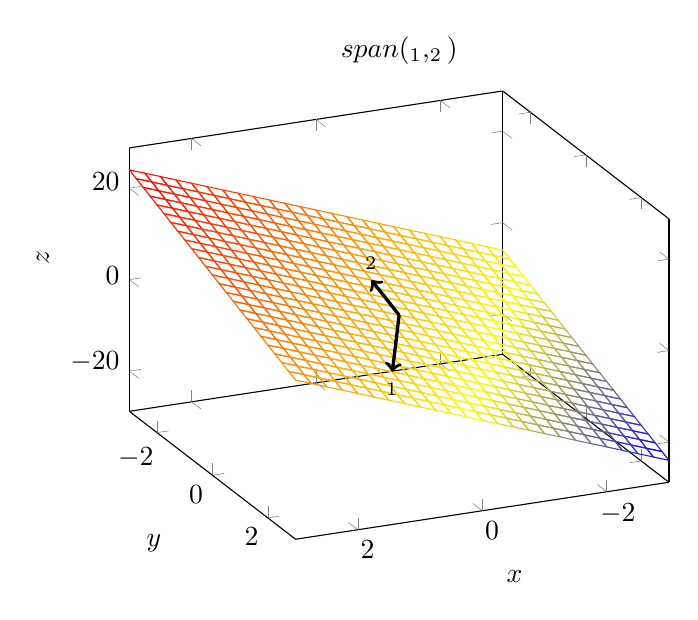
\begin{tikzpicture}
            \begin{axis}[ title={$\text{span}(\bv_1,\bv_2)$}, view={156}{28}, domain=-3:3,
                xlabel={$x$}, ylabel={$y$}, zlabel={$z$}]
                \addplot3[mesh] {5*x-3*y};
                \draw[very thick,->] (axis cs:0,0,0) -- (axis cs:1,2,-1) node[anchor=north]{$\bv_1$};
                \draw[very thick,->] (axis cs:0,0,0) -- (axis cs:0,-1,3) node[anchor=south]{$\bv_2$};
            \end{axis}
        \end{tikzpicture}
    \end{center}
    \caption{The span of $\bv_1$ and $\bv_2$ in $\mathbb{R}^3$.}
    \label{fig:10.5.span}
\end{figure}

% \input{activities/10.5.IndDep.Act1.tex}
\begin{problem}
    In each of the following, determine if $\bw$ is in the span of the other vectors.  If
    it is then express $\bw$ as a linear combination of the other vectors.
\ba
    \item $\bv_1=\bpm 2\\-1\epm$, $\bv_2=\bpm 2\\1\epm$, and $\bw=\bpm 5\\3\epm$. (Use the
        applet
        \href{http://tube.geogebra.org/student/m1254137}{http://tube.geogebra.org/student/m1254137}
        to visualize this problem)
    \item $\bv_1 = \bpm 1\\-2\\0\epm$, $\bv_2=\bpm0\\1\\2\epm, \bv_3=\bpm5\\-6\\8\epm$,
        and $\bw = \bpm2\\-1\\6\epm$.
\ea
\end{problem}

\newpage\section{Linear Independence, Linear Dependence, and Basis}
The span of the vectors $\bu = (1,0)^T$ and $\bv = (0,1)^T$ is the entire two dimensional
plane $\mathbb{R}^2$.  This means that if we have a vector in $\mathbb{R}^2$, say $\bx =
(3,5)^T$ then we know that it can be written as a linear combination of the vectors $\bu$
and $\bv$:
\[ \bpm 3\\5\epm = 3 \bpm 1\\0\epm + 5 \bpm 0\\1\epm. \]
The vector $\bx = (3,5)^T$ can be built from the vectors $\bu$ and $\bv$ so, in some
sense, $\bx$ {\it depends} on $\bu$ and $\bv$.  We would say that the set of vectors
$\{\bu,\bv,\bx\}$ is {\it linearly dependent} since one of the vectors in the set can be
built from linear combinations of the others.  The set $\{\bu,\bv\}$ is called {\it
linearly independent} since none of the vectors in the set can be built from linear
combinations of the other vectors in the set.
\begin{definition}
    A collection of vectors $\{\bv_1, \bv_2, \dots, \bv_p\}$ in $\mathbb{R}^n$ is called {\bf linearly
    independent} if the vector equation
    \[ c_1 \bv_1 + c_2 \bv_2 + \cdots c_p \bv_p = \texttt{0} \]
    has {\it only} the trivial solution $c_1=0, c_2=0, \dots, c_p=0$.
\end{definition}

\begin{definition}
    A collection of vectors $\{\bv_1, \bv_2, \dots, \bv_p\}$ is called {\bf linearly
    dependent} if it is not linearly independent.
\end{definition}


\begin{example}
Determine whether or not the vectors $\bv_1$, $\bv_2$, and $\bv_3$ are linearly independent or
dependent.
\[ \bv_1 = \begin{pmatrix} 1 \\ 2 \\ 3 \end{pmatrix} \quad \bv_2 = \begin{pmatrix} 3 \\ -2 \\
    0 \end{pmatrix} \quad \bv_3 = \begin{pmatrix} 4 \\ 1 \\ 1 \end{pmatrix} \]
{\bf Solution:} 
To determine if $\bv_1, \bv_2,$ and $\bv_3$ are linearly independent or not we need to
consider the equation
\[ c_1 \bv_1 + c_2 \bv_2 + c_3 \bv_3 = \bo. \]
If the solution to this equation is that $c_1 = c_2 = c_3 = 0$ then the vectors will be
linearly independent.  Otherwise they will be linearly dependent.  This can be viewed as a
question about the solutions to the following system of equations (which we will write in
several different ways):
\[ c_1 \begin{pmatrix} 1 \\ 2 \\ 3 \end{pmatrix} + c_2 \begin{pmatrix} 3 \\ -2 \\ 0
    \end{pmatrix} + c_3 \begin{pmatrix} 4 \\ 1 \\ 1 \end{pmatrix} = \begin{pmatrix} 0 \\
    0 \\ 0 \end{pmatrix}, \]
which is the same as 
\[ \left\{ \begin{array}{cl} c_1 + 3c_2 + 4c_3 &= 0 \\ 2c_1 - 2c_2 + c_3 &= 0 \\ 3c_1 +
    c_3 &= 0 \end{array} \right. \]
which is the same as the augmented matrix
\[ \left( \begin{array}{ccc|c} 1 & 3 & 4 & 0 \\ 2 & -2 & 1 & 0 \\ 3 & 0 & 1 & 0 \end{array}
\right) \]
Row reducing the augmented form gives us
\[ \left( \begin{array}{ccc|c} 1 & 0 & 0 & 0 \\ 0 & 1 & 0 & 0 \\ 0 & 0 & 1 & 0 \end{array}
\right). \]
Hence, we can see that the solution to the system of equations is $c_1 = c_2 = c_3 = 0$.
This implies that $\bv_1, \bv_2,$ and $\bv_3$ are linearly independent.
\end{example}

Now let's look at one more example.
\begin{example}
Determine whether or not the vectors $\bv_1$, $\bv_2$, and $\bv_3$ are linearly independent or
dependent.
\[ \bv_1 = \begin{pmatrix} 1 \\ 2 \\ 3 \end{pmatrix} \quad \bv_2 = \begin{pmatrix} 3 \\ -2 \\
    0 \end{pmatrix} \quad \bv_3 = \begin{pmatrix} 4 \\ 0 \\ 3 \end{pmatrix} \]
{\bf Solution:}
We'll start by writing the system of equations $c_1 \bv_1 + c_2 \bv_2 + c_3 \bv_3 = \bo$
in multiple ways just as we did before.
\[ c_1 \begin{pmatrix} 1 \\ 2 \\ 3 \end{pmatrix} + c_2 \begin{pmatrix} 3 \\ -2 \\ 0
    \end{pmatrix} + c_3 \begin{pmatrix} 4 \\ 0 \\ 3 \end{pmatrix} = \begin{pmatrix} 0 \\
    0 \\ 0 \end{pmatrix} \text{ or } \quad \left\{ \begin{array}{cl} c_1 + 3c_2 + 4c_3 &= 0 \\ 2c_1 - 2c_2  &= 0 \\ 3c_1 +
    3c_3 &= 0 \end{array} \right. \text{ or } \quad  \left( \begin{array}{ccc|c} 1 & 3 & 4 & 0 \\ 2 & -2 & 0 & 0 \\ 3 & 0 & 3 & 0 \end{array}
\right) \]
Row reducing the augmented form gives us
\[ \left( \begin{array}{ccc|c} 1 & 0 & 1 & 0 \\ 0 & 1 & 1 & 0 \\ 0 & 0 & 0 & 0 \end{array}
\right). \]
Now we can see that there are infinitely many solutions to the equation $c_1 \bv_1 + c_2
\bv_2 + c_3 \bv_3 = \bo$ and so the vectors $\bv_1, \bv_2,$ and $\bv_3$ are linearly
dependent. 

Moreover, we can see that $c_1 + c_3 = 0$ and $c_2 + c_3 = 0$.  We can rewrite these
equations as $c_1 = -c_3$ and $c_2 = -c_3$, and therefore $c_1, c_2$ and $c_3$ must
satisfy the equation
\[ \begin{pmatrix} c_1 \\ c_2 \\ c_3 \end{pmatrix} = \begin{pmatrix} -1 \\ -1 \\ 1
\end{pmatrix} t, \quad \text{for} \quad t \in \mathbb{R}. \]
The fact that there are infinitely many solutions to the system of equations further
illustrates the idea that the vectors $\bv_1, \bv_2$ and $\bv_3$ are linearly dependent:
the coefficients of $c_1$ and $c_2$ \underline{depend} on the value for $c_3$.
\end{example}



% 
% \input{activities/10.5.IndDep.Act2.tex}
\begin{problem}
Use the definitions of linearly independent and linearly dependent to answer the following
questions.
    \ba
        \item Are the vectors $\bv_1= \bpm 1 \\ 0 \epm$ and $\bv_2=\bpm 0\\1\epm$ linearly
            independent or dependent? Explain.
        \item Are the vectors $\bv_1= \bpm 1 \\ 2 \epm$ and $\bv_2=\bpm 3\\6\epm$ linearly
            independent or dependent? Explain.
        \item Are the vectors $\bv_1 = \bpm 1\\0\\-3\epm, \bv_2 = \bpm 3\\1\\-4\epm,
            \bv_3=\bpm-2\\-1\\1\epm,$ and $\bv_4=\bpm2\\-1\\1\epm$ linearly independent or
            dependent?  Explain.
        \item If nonzero vectors $\bv_1$ and $\bv_2$ in $\mathbb{R}^2$ only span a line in
            $\mathbb{R}^2$ are they linearly independent or linearly dependent?
        \item If nonzero vectors $\bv_1$, $\bv_2$ and $\bv_3$ in $\mathbb{R}^3$ span all
            of $\mathbb{R}^3$ are they linearly independent or linearly dependent?
    \ea

\end{problem}

Loosely speaking, linear independence means that no vector in the collection can be {\it
built} from the other vectors in the collection.   Linearly dependence, on the other hand,
means that at least one vector can be built from the other vectors in the collection.  The
real beauty of linearly independent sets is that they can serve as very simple descriptors
of a much larger set.  For example, the vectors $\bpm 1\\0\epm$ and $\bpm 0\\1\epm$ are
linearly independent (as seen in the previous activity) and the span of these two simple
vectors is all of $\mathbb{R}^2$.  These two facts together mean that $\bpm1\\0\epm$ and
$\bpm0\\1\epm$ are the simplest building blocks for the entire $xy$-plane; there is no
unneeded information and there is enough to build every point.  In some sense, these two
vectors are the DNA of the $xy$-plane.

There are many other
linearly independent spanning sets for $\mathbb{R}^2$ but the amazing fact is that they
all have exactly 2 vectors in them.  Similarly, all of the linearly independent spanning
sets of $\mathbb{R}^3$ will all contain exactly 3 vectors.  In fact, this is where our
intuitive notion of dimensionality comes from; the number of vectors in the linearly
independent spanning set.

\begin{definition}
    If the set of vectors $\mathcal{B} = \{\bb_1, \bb_2, \dots, \bb_p \}$ spans a space
    $V$ then $\mathcal{B}$ is said to be a {\bf basis} of $V$ if it is linearly
    independent.  In other words, a basis is a linearly independent spanning set.
\end{definition}


\begin{example}
Show that $\mathcal{B} = \left\{ \bpm 1\\2\epm, ~ \bpm -1\\1\epm\right\}$ is a basis for
$\mathbb{R}^2$.
\\{\bf Solution:}
We first need to show that $\mathcal{B}$ is linearly independent.  This means that we need
to show that the equation $c_1 \bb_1 + c_2 \bb_2 = \bo$ has only the trivial solution
$c_1=c_2=0$.  Indeed,
\begin{flalign*}
    &c_1 \bpm 1\\2\epm + c_2 \bpm-1\\1\epm = \bpm0\\0\epm \\
    &\implies \bpm 1 & -1 \\ 2 & 1 \epm \bpm c_1 \\ c_2 \epm = \bpm 0 \\ 0 \epm \\
    &\implies \left( \begin{array}{cc|c} 1 & -1 & 0 \\ 2 & 1 & 0 \end{array} \right) \to
    \cdots \to \left( \begin{array}{cc|c} 1 & 0 & 0 \\ 0 & 1 & 0 \end{array} \right) \\
    &\implies c_1 = c_2 = 0.
\end{flalign*}
Hence, $\mathcal{B}$ is a linearly independent set.

To show that $\mathcal{B}$ spans $\mathbb{R}^2$ we need to show that any vector $\bpm
x\\y\epm$ can be {\it built} as a linear combination of the vectors in $\mathcal{B}$.
Indeed,
\begin{flalign*}
    &c_1 \bpm 1\\2\epm + c_2 \bpm-1\\1\epm = \bpm x\\y\epm \\
    &\implies \bpm 1 & -1 \\ 2 & 1 \epm \bpm c_1 \\ c_2 \epm = \bpm x \\ y \epm \\
    &\implies \left( \begin{array}{cc|c} 1 & -1 & x \\ 2 & 1 & y \end{array} \right) \to
    \cdots \to \left( \begin{array}{cc|c} 1 & 0 & \frac{x+y}{3} \\ 0 & 1 &
        \frac{-2x+y}{3} \end{array} \right) \\
    &\implies c_1 = \frac{x+y}{3} \quad \text{and} \quad c_2 = \frac{-2x+y}{3}.
\end{flalign*}
Hence, given {\bf any} point in the $xy$-plane we can find $c_1$ and $c_2$ that will
build the point as a linear combination of vectors in $\mathcal{B}$.  Therefore,
$\mathcal{B}$ is a basis for $\mathbb{R}^2$.
\end{example}


\begin{example}
Is $\mathcal{B} = \left\{ \begin{pmatrix} 1\\2\end{pmatrix} , \begin{pmatrix}
    2\\4\end{pmatrix} \right\}$ a basis for $\mathbb{R}^2$?
\\{\bf Solution:}
No. The reader should verify that the two vectors in $\mathcal{B}$ are linearly dependent
so they cannot possible span all of $\mathbb{R}^2$.
\end{example}

% 
% \input{activities/10.5.IndDep.Act3.tex}
\begin{problem}
\ba
    \item Find a basis for the set of vectors in $\mathbb{R}^2$ on the line $y=3x$.
    \item Find a basis for the space spanned by the vectors $\bv_1, \dots, \bv_5$.
        \[ \bv_1 = \bpm 1\\0\\-2\\3\epm, \quad \bv_2 = \bpm 0\\1\\2\\3\epm, \quad \bv_3 =
            \bpm 2\\-2\\-8\\0\epm, \quad \bv_4=\bpm2\\-1\\10\\3\epm, \quad \bv_5=\bpm
        3\\-1\\-6\\9\epm.\]
        (Use technology to complete this exercise to save a bit of time)
    \item Let $\bv_1 = \bpm4\\-3\\7\epm$, $\bv_2=\bpm 1\\9\\-2\epm$, and $\bv_3=\bpm
        7\\11\\6\epm$, and also let $H = \text{span}(\{\bv_1,\bv_2,\bv_3\})$.  It can be
        verified that $4\bv_1 + 5\bv_2 - 3\bv_3 = \bo$.  Use this information to find a
        basis for $H$.  (There is more than one answer)
\ea

\end{problem}


% 
% \input{activities/10.5.IndDep.Act4.tex}
\begin{problem}
    Mark each statement as True or False.  Justify each answer.
\ba
\item A single vector by itself is linearly dependent.
\item If $H = \text{span}(\{\bb_1, \dots, \bb_p\})$ then $\{\bb_1, \dots, \bb_p\}$ is a
    basis for $H$.
\item The columns of an invertible $n \times n$ matrix form a basis for $\mathbb{R}^n$.
\item A basis is a spanning set that is as large as possible.
\item Any linearly independent set in a space $V$ is a basis for $V$.
\item If a finite set $S$ of nonzero vectors spans a space $V$, then some subset of $S$ is
    a basis for $V$.
\item A basis is a linearly independent set that is as large as possible.
\ea

\end{problem}
% 
\newpage\section{The Column and Null Spaces of a Matrix}
For any matrix there are several fundamental spaces that fully describe the actions that a
matrix can have on a vector.  The two that we focus on here are the column space and the
null space.

\begin{definition}
    The {\bf column space} of a matrix $A$ is the space that is spanned by the columns of the
    matrix.
\end{definition}

\begin{definition}
    The {\bf null space} of an $m \times n$ matrix $A$, written $\text{Nul}(A)$, is the
    set of all solutions of the homogeneous equation $A\bx=\bo$.
\end{definition}

\begin{example}
Find the null and column spaces of the matrix 
\[ A = \bpm 1 & -3 & -2 \\ -5 & 9 & 1 \epm \]
and determine if $\bu = \bpm 5\\3\\-2\epm$ belongs to the null space of $A$.
\\{\bf Solution:}
The column space of $A$ is the space spanned by the columns of $A$.  We need to determine
if the three columns are linearly independent.  Row reduction shows us that
\[ \bpm 1 & -3 & -2 \\ -5 & 9 & 1 \epm \to \cdots \to \bpm 1 & 0 & \frac{5}{2} \\ 0 & 1 &
\frac{3}{2} \epm \]
so the third column vector depends on the other two.  Hence, there are two linearly
independent vectors that form a basis for the column space.  Since each vector is in
$\mathbb{R}^2$ we see that the column space is all of $\mathbb{R}^2$.

The null space of $A$ is the set of solutions to $A\bx =\bo$. We have already row reduced
the homogeneous system so we know that $x_1 = -5/2 x_3$ and $x_2 = -3/2 x_3$.  Hence, if
$x_3 = t$ then
\[ \bx = \bpm -5/2 t \\ -3/2 t \\ t \epm = \bpm -5/2 \\ -3/2 \\ 1 \epm t \]
where $t$ is any real number.

Clearly, if we take $t=-2$ then $\bx = \bpm 5\\3\\-2 \epm$ showing that $\bu$ is in the
null space of $A$.  Another (simpler) way to see that $\bu$ is in the null space of $A$ is
to observe that 
\[ A\bu = \bpm 1&-3&-2\\-5&9&1\epm \bpm 5\\3\\-2\epm = \bpm 5-9+4 \\ -25+27-2\epm =
\bpm0\\0\epm.\]
\end{example}

% \input{activities/10.5.IndDep.Act5.tex}
\begin{problem}
Find the null and column spaces for the matrix 
\[ A = \bpm -2 & 4 & -2 & -4 \\ 2 & -6 & -3 & 1 \\ -3 & 8 & 2 & -3 \epm. \]
The matrix $A$ is $3 \times 4$.  Be sure to specify where the null and column spaces

\end{problem}



\newpage\section{Modeling Explorations with Linear Algebra}
In 1973, Wassily Leontief was awarded the Nobel prize for his work in economics.  Part of
his work was to apply the basic concepts of linear algebra to model supply and demand
within simple economies.  His theory, called the Leontief Input Output model, serves as a
simplified model to predict production.

% \input{previews/10.5.PA1}
\begin{lab}\label{PA:10.5}
    Suppose that an economy is divided into three sectors: manufacturing, agriculture, and
    services.  Let $\bx$ be a $3 \times 1$ vector (called the {\it production vector})
    that lists the outputs of each sector for one year.  At the same time, let $\texttt{d}$ be a
    $3 \times 1$ vector (called the {\it demand vector}) that lists any external demands
    on the goods and services from the non productive part of the economy (consumer
    demand, government consumption, exports, etc.)   

    As the three sectors produce goods to meet consumer demand, the producers themselves
    create additional {\it intermediate demand} for goods they need as inputs for their
    own production.  For example, the agriculture sector will use equipment made by the
    manufacturing sector. The basic question Leontief asked is ``is there a production
    level $\bx$ such that the amounts produced will exactly balance the total demand for
    the production?'' In other words, find $\bx$ so that
    \[ \underbrace{\text{amount produced}}_{\bx} = \underbrace{\text{intermediate
    demand}}_{C\bx} + \underbrace{\text{external demand}}_{\texttt{d}}. \]
    Here we take $C$ to be a matrix defining unit consumptions of the various sectors (see
    the table).

    \begin{center}
        \begin{tabular}{lccc}
            \hline
            & \multicolumn{3}{c}{Inputs per Unit of Output} \\ 
            {\bf Purchased From:} & {\bf Manufacturing} & {\bf Agriculture} & {\bf
            Services} \\ \hline \hline
            {\bf Manufacturing} &0.50  &0.40  &0.20  \\
            {\bf Agriculture} &0.20  &0.30  &0.10  \\
            {\bf Services} & 0.10 &0.10  &0.30  \\ \hline
        \end{tabular}
    \end{center}

    In the table, the columns read as follows:
    \begin{itemize}
        \item To produce 1 unit, manufacturing needs 0.50 units from other parts of
            manufacturing, 0.20 units from agriculture, and 0.10 units from services.
        \item To produce 1 unit, agriculture needs 0.40 units from manufacturing, 0.30
            units from other parts of agriculture, and 0.10 units from services.
        \item To produce 1 unit, services need 0.20 units from manufacturing, 0.10 units
            from agriculture, and 0.30 units from other services.
    \end{itemize}

    Suppose that the external demand is 50 units for manufacturing, 30 units for
    agriculture, and 20 units for services.
    \ba
        \item If the production is 
            \[ \bx = \bpm 140 \\ 20 \\ 50 \epm \]
            then what is the sum of the intermediate demand and the external demand?  Did
            the economy under or over produce in each of the sectors?
        \item We want to find the production $\bx$ that gives a perfectly balance
            economy: $\bx = C \bx + \texttt{d}$.  How do we solve this matrix equation?
    \ea
\end{lab}

\subsection{Input-Output Economies}
In the previous problem we explored situations where a simple economy over
or under produces.  Theoretically, a perfectly functioning economy has no surplus or
shortage.  We would like to explore Leontief's original question and determine if there is
a perfect production level that will yield no surplus or shortage.  

The matrix equation associated with the Leontif Input Output model is 
\begin{flalign}
    \bx = C \bx + \texttt{d}.
    \label{eqn:10.5.inout1}
\end{flalign}
The trouble is that the production level, $\bx$, shows up on both sides of the matrix
equation.  To overcome this fact we do a few simple steps of matrix arithmetic to equation
\eqref{eqn:10.5.inout1}:
\begin{flalign}
    \bx = C \bx + \texttt{d} \quad \implies \quad \bx - C\bx = \texttt{d} \quad \implies \quad \left(
    I - C \right) \bx = \texttt{d} \quad \implies \quad \bx = \left( I - C \right)^{-1} \texttt{d}.
    \label{eqn:10.5.inout2}
\end{flalign}
The right-hand equation of \eqref{eqn:10.5.inout2} shows that there is a ready-made
formula that allows us to solve for the production level.

\begin{example}
Solve for the optimal production level using the internal and external demands from
Problem \ref{PA:10.5}.
\\{\bf Solution:}
We want to find the production level $\bx$ given that the consumption matrix $C$ and the
demand vector $\texttt{d}$ are 
\[ C = \bpm 0.5 & 0.4 & 0.2 \\ 0.2 & 0.3 & 0.1 \\ 0.1 & 0.1 & 0.3 \epm \quad \text{and}
    \quad \texttt{d} = \bpm 50 \\ 30 \\ 20 \epm. \]
From equation \eqref{eqn:10.5.inout2} we need to solve the equation $(I-C) \bx = \texttt{d}$ by
evaluating $\bx = (I-C)^{-1} \texttt{d}$. 

It is impractical to actually compute the inverse\footnote{In the vast majority of linear
algebra applications the inverse is never computed.}, so instead we can create an
augmented matrix $(I-C \, | \, \texttt{d})$ and use row reduction.
\[ (I-C \, | \, \texttt{d}) = \left( \begin{array}{ccc|c} 0.5 & -0.4 & -0.2 & 50 \\ -0.2 & 0.7 &
        -0.1 & 30 \\ -0.1 & -0.1 & 0.7 & 20 \end{array} \right) \to \cdots \to \left(
        \begin{array}{ccc|c} 1 & 0 & 0 & 225.9 \\ 0 & 1 & 0 & 118.5 \\ 0 & 0 & 1 & 77.8
        \end{array} \right). \]
Hence, in this economy, manufacturing must produce approximately 226 units, agriculture
must produce approximately 119 units, and services must produce approximately 78 units.
This will lead to a balanced economy where this is no surplus or shortage.
\end{example}

% \input{activities/10.5.Act1}
\begin{lab}
    The consumption matrix $C$ below is based on input-output data for the U.S. economy in
    1958, with data for 81 sectors grouped into 7 larger sectors: 
    \begin{enumerate}
        \item nonmetal household and personal products,
        \item final metal products (such as motor vehicles),
        \item basic metal products and mining,
        \item basic nonmetal products and agriculture,
        \item energy,
        \item services, and
        \item entertainment and miscellaneous products.
    \end{enumerate}
   
    \[ C = \bpm 0.1588 & 0.0064 & 0.0025 & 0.0304 & 0.0014 & 0.0083 & 0.1594 \\
                0.0057 & 0.2645 & 0.0436 & 0.0099 & 0.0083 & 0.0201 & 0.3414 \\
                0.0264 & 0.1506 & 0.3557 & 0.0139 & 0.0142 & 0.0070 & 0.0236 \\
                0.3299 & 0.0565 & 0.0495 & 0.3636 & 0.0204 & 0.0483 & 0.0649 \\
                0.0089 & 0.0081 & 0.0333 & 0.0295 & 0.3412 & 0.0237 & 0.0020 \\
                0.1190 & 0.0901 & 0.0996 & 0.1260 & 0.1722 & 0.2368 & 0.3369 \\
                0.0063 & 0.0126 & 0.0196 & 0.0098 & 0.0064 & 0.0132 & 0.0012
        \epm, \quad \texttt{d} = \bpm 74000\\56000\\10500\\25000\\17500\\196000\\5000 \epm \]

% The following are the data sets in MATLAB format.
%    C = [.1588 .0064 .0025 .0304 .0014 .0083 .1594;.0057 .2645 .0436 .0099 .0083 .0201 .3413;.0264 .1506 .3557 .0139 .0142 .0070 .0236;
%         .3299 .0565 .0495 .3636 .0204 .0483 .0649;.0089 .0081 .0333 .0295 .3412 .0237 .0020;.1190 .0901 .0996 .1260 .1722 .2368 .3369;
%         .0063 .0126 .0196 .0098 .0064 .0132 .0012], 
%    d = [74000;56000;10500;25000;17500;196000;5000]
%    d = [99640;75548;14444;33501;23527;263985;6526]
    \ba
        \item Use technology to find the production levels needed to satisfy the final
            demand $\texttt{d}$.
        \item The demand in 1964 was 
            \[ \texttt{d} = \bpm 99640&75548&14444&33501&23527&263985&6526 \epm^T \]
            Find the production levels needed to satisfy this demand.
        \item In the six years between 1958 and 1964 the demand changed drastically in
            several categories leading to changes in the production levels.  Use the data
            in this problem to extrapolate to current demands and production levels.  Give
            several reasons why your extrapolation will ultimately give poor estimates.
    \ea
\end{lab}

\subsection{Traffic Networks}
A traffic network can be viewed as a collection of lines (streets) and intersections.
When modeling a large street network, the influx from certain suburbs and other cities is
generally well known.  To estimate the number of cars on given streets, traffic engineers
often put counters at the intersections.  This allow them to calculate flow given that
\[ \text{flow into an intersection} = \text{flow out of an intersection}. \]
This simple {\it conservation law} creates a system of equations for all of the streets
that can be solved to find the flow on each individual street.

% \input{activities/10.5.Act2}
\begin{lab}
Consider the collection of one-way streets in a downtown area.

\begin{center}
    \begin{tikzpicture}
        \draw[thick,->] node[anchor=east]{$200$} (0,0) -- (2,0);
        \draw[thick,->] (2,0) -- (5,0);
        \draw[thick,->] (5,0) -- (7,0);
        \draw[thick,->] (7,0) -- (9,0) node[anchor=west]{$500$};
        \draw[fill=black] (3,0) circle(0.07cm) node[anchor=north west]{$A$};
        \draw[fill=black] (6,0) circle(0.07cm) node[anchor=north west]{$B$};
        %
        \draw (0,3) node[anchor=east]{$300$}; 
        \draw[thick,<-] (0,3) -- (2,3);
        \draw[thick,<-] (2,3) -- (5,3);
        \draw[thick,<-] (5,3) -- (7,3);
        \draw[thick,<-] (7,3) -- (9,3) node[anchor=west]{$400$};
        \draw[fill=black] (3,3) circle(0.07cm) node[anchor=north west]{$C$};
        \draw[fill=black] (6,3) circle(0.07cm) node[anchor=north west]{$D$};
        %
        \draw (3,-2) node[anchor=north]{$500$};
        \draw[thick,->] (3,-2) -- (3,-1);
        \draw[thick,->] (3,-1) -- (3,2);
        \draw[thick,->] (3,2) -- (3,5);
        \draw (3,5) node[anchor=south]{$x_3$};
        %
        \draw (6,-2) node[anchor=north]{$50$};
        \draw[thick,<-] (6,-2) -- (6,-1);
        \draw[thick,<-] (6,-1) -- (6,2);
        \draw[thick,<-] (6,2) -- (6,5);
        \draw[thick,<-] (6,4) -- (6,5);
        \draw (6,5) node[anchor=south]{$100$};
        %
        \draw (4.5,0) node[anchor=north]{$x_1$};
        \draw (4.5,3) node[anchor=north]{$x_4$};
        \draw (3,1.5) node[anchor=west]{$x_2$};
        \draw (6,1.5) node[anchor=east]{$x_5$};
    \end{tikzpicture}
\end{center}

\ba
    \item Fill in the table for each intersection.  The first line has been done to get
        you started.
        \begin{center}
            \begin{tabular}{ccc}
                Intersection & Flow In & Flow Out \\ \hline \hline
                $A$ & $200 + 500$ & $x_1 + x_2$ \\
                $B$ & & \\
                $C$ & & \\
                $D$ & & \\ \hline
            \end{tabular}
        \end{center}

    \item Write the equation
        \[ \text{total flow into the network} = \text{total flow out of the network}. \]
        This equation describes the fact that the network is not closed but the number of
        cars in the network must be conserved (just like conservation of mass or
        momentum from physics).
    \item Use parts (a) and (b) to write a system of equations.  Solve the system to
        determine the traffic flow at $x_1$, $x_2$, \dots, $x_5$.
    \item {\bf Sensitivity Analysis:} There are 7 different given values in this network.
        What is the percent change in each of the variables $x_1,\dots, x_5$ if each of
        the given values were to increase or decrease by 10\%?  Use a table like the one
        below to help organize the results, and use your results to write a short report
        to the traffic division.\\ Hint: Test each value one at a time.

        \begin{center}
            \begin{tabular}{|c|c||c|c|c|c|c|}
                \hline
                & & \multicolumn{5}{|c|}{Percent Change} \\ \hline
                Old Value & New Value & $x_1$ & $x_2$ & $x_3$ & $x_4$ & $x_5$ \\ \hline
                \hline
                100 & 110 & & & & & \\\hline
                100 & 90 & & & & & \\\hline\hline
                400 & 440 & & & & & \\\hline
                400 & 360 & & & & & \\\hline\hline
                500 & 550 & & & & & \\\hline
                500 & 450 & & & & & \\\hline\hline
                50 & 55 & & & & & \\\hline
                50 & 45 & & & & & \\\hline\hline
                500 & 550 & & & & & \\\hline
                500 & 450 & & & & & \\\hline\hline
                200 & 220 & & & & & \\\hline
                200 & 180 & & & & & \\\hline\hline
                300 & 330 & & & & & \\\hline
                300 & 270 & & & & & \\\hline
            \end{tabular}
        \end{center}
\ea

\end{lab}


% \input{activities/10.5.Act3}
\begin{lab}
Your boss at the trucking company wants you to solve the following traffic flow problem.
In this problem, the lettered nodes are distribution centers for your trucking company and
the numbers and variables along the arcs are the truck flows in a given year.  Remember
that for each distribution center
\[ \text{yearly flow into the distribution center} = \text{yearly flow out of the
distribution center}. \]
For example, at node $H$ we must have $x_{FH} = x_{HS}+x_{HM}+600$. \\Hint: write an
equation for each node and then rearragne into an augmented system of equations.

Your goal is to find the roads with the maximum truck volume and to perform a sensitivity
analysis on the known information in the problem (i.e. if each known value were to change
by as much as 10\%, how much would the maximum road volume change).  Give advice to your
boss based on your analysis keeping in mind that the highway department would ultimately
like to minimize the maximum truck volume on the roads.
% If the flow prescribed is impossible be sure to state why. If there is more than one
% unique solution then give advice to your boss about how to choose an appropriate solution
% so that no center accumulates more trucks than they send.
\begin{center}
    \begin{tikzpicture}[scale=0.75,transform shape]
        \Vertex[x=0,y=0]{K}
        \Vertex[x=-3,y=2.5]{F}
        \Vertex[x=-1,y=4]{D}
        \Vertex[x=3,y=7]{H}
        \Vertex[x=8,y=5]{B}
        \Vertex[x=11,y=3]{N}
        \Vertex[x=5,y=-0.5]{M}
        \Vertex[x=3,y=2]{S}
        \tikzstyle{LabelStyle}=[fill=white,sloped]
        \tikzstyle{EdgeStyle}=[post,bend left]
        \Edge[label=$x_{KF}$](K)(F)
        \Edge[label=$x_{HM}$](H)(M)
        \Edge[label=$x_{NB}$](N)(B)
        \Edge[label=$x_{DB}$](D)(B)
        \Edge[label=$300$](M)(D)
        \Edge[label=$780$](B)(M)
        \Edge[label=$600$](H)(N)
        \Edge[label=$x_{FH}$](F)(H)
        \Edge[label=$520$](M)(K)
        \Edge[label=$x_{NS}$](N)(S)
        \Edge[label=$450$](S)(K)
        \Edge[label=$x_{DF}$](D)(F)
        \tikzstyle{EdgeStyle}=[post, bend right]
        \Edge[label=$x_{SB}$](S)(B)
        \Edge[label=$x_{SM}$](S)(M)
        \Edge[label=$x_{HS}$](H)(S)
    \end{tikzpicture}
\end{center}
\end{lab}


\subsection{Balancing Chemical Equations}
The final application that we will discuss here is that of balancing chemical equations.  

Consider the chemical reaction: Nitrogen Dioxide plus water yields Nitrous acid and Nitric
acid.
\[ aNO_2 + b H_2O \to c HNO_2 + d HNO_3 \]
The coefficients $a,b,c$, and $d$ are unknown positive integers.  The reaction must be
balanced; that is, the number of atoms of each element must the same before and after the
reaction.  Because the number of atoms must remain the same we end up with the following
system of equations:
\begin{align*}
    &\text{Oxygen: } &  2a + b &= 2c + 3d \\
    &\text{Nitrogen: }  & a &= c + d \\
    &\text{Hydrogen: }  & 2b &= c + d
\end{align*}
Rearranging this into an augmented system gives the homogeneous system
\[ \left( \begin{array}{cccc|c} 2 & 1 & -2 & -3 & 0 \\
                                1 & 0 & -1 & -1 & 0 \\
                                0 & 2 & -1 & -1 & 0 \end{array} \right) \]
Performing row reductions on this system gives
\[ \left( \begin{array}{cccc|c} 2 & 1 & -2 & -3 & 0 \\
                                1 & 0 & -1 & -1 & 0 \\
                                0 & 2 & -1 & -1 & 0 \end{array} \right) 
    \to
   \left( \begin{array}{cccc|c} 1 & 0 & -1 & -1 & 0 \\
                          0 & 1 & 0 & -1 & 0 \\
                          0 & 2 & -1 & -1 & 0 \end{array} \right)
    \to
   \left( \begin{array}{cccc|c} 1 & 0 & -1 & -1 & 0 \\
                          0 & 1 & 0 & -1 & 0 \\
                          0 & 0 & -1 & 1 & 0 \end{array} \right)
                                \]
\[ \to 
   \left( \begin{array}{cccc|c} 1 & 0 & 0 & -2 & 0 \\
                          0 & 1 & 0 & -1 & 0 \\
                          0 & 0 & 1 & -1 & 0 \end{array} \right)
    \quad \implies \quad \begin{array}{l} a=2d \\ b=d \\ c=d \end{array}
                                \]
In this chemical equation we see that $d$, the coefficient of Nitric acid, is a free
variable.  Mathematically this means that we can freely choose $d$ to be any value we
like, but scientifically we choose the smallest positive integer: $d=1$.  Hence
\[ a=2, \quad b=1, \quad c=1, \quad \text{and} \quad d=1 \]
so the balanced chemical equation becomes
\[ 2NO_2 + H_2O \to HNO_2 + HNO_3 \]

% \input{activities/10.5.Act4}
\begin{lab}
Find the lower case values that balance each of the chemical equations.
\ba
    \item Aluminum oxide and carbon react to create elemental aluminum and carbon dioxide:
        \[ a Al_2O_3 + b C \to c Al + d CO_2. \]
    \item Limestone, $CaCO_3$, netralizes the acid, $H_3O$, in acid rain by following the
        equation
        \[ a H_3O + b CaCO_3 \to c H_2O + d Ca + e CO_2. \]
    \item Boron sulfide reacts violently with water for form boric acid and hydrogen
        sulfide gas (the smell of rotten eggs). 
        \[ a B_2 S_3 + b H_2O \to c H_3 BO_3 + d H_2 S \]
\ea
\end{lab}
